\chapter{Materials and methods}\label{chap:MatlsMethds}
A series of batch shaking tests was conducted to test the sorption strength of waste-based biochars to PFAS, and to determine possible sorption mechanisms. Experiments were conducted using six perfluorinated carboxylic acids (PFCAs) (C5-C10) to investigate how chain length affects sorption, both with and without the presence of soil. Both single compound and a cocktail of C5-C10 batch tests were performed to determine attenuation factors. A methods flowchart is given in \cref{fig:methodoverview}. The main work and laboratory experiments were conducted in the environmental chemistry laboratory at the Norwegian Geotechnical Institute (NGI), Oslo. The quantification analysis of the batch test filtrates was performed by LC-MS/MS at the Institute for Chemistry, Norwegian University of Science and Technology (NTNU), Trondheim. 

\section{Feedstock}
Three feedstocks were selected for use as sorbents for the sorption experiments:

\begin{itemize}
    \item \textbf{Ullensaker sludge (ULS)}: raw sewage sludge biosolids from Ullensaker wastewater treatment plant located North-East of Oslo, Norway. 
    \item \textbf{Digested sludge Lindum (DSL)}: the remaining solid residue (digestate) after anaerobic digestion of sludge from food waste and organic material used to produce commercial biogas performed at Lindum AS (Drammen, Norway). Anaerobic digestion produces mainly methane by the reaction: 
        \begin{equation}
        \label{eq:AD}
            \ce{C_cH_hO_oN_nS_s + yH_2O -> xCH_4 + nNH_3 + xH_2S + (c-x)CO_2}
        \end{equation}
    \item \textbf{Clean wood chips (CWC)}: clean, fresh softwood timber without additives that has been shredded, dried, and compressed into 8 mm pellets. The wood pellets are commercially available from Hallingdal Trepellets (Kleivi næringspark, Ål)
\end{itemize}

These feedstocks were dried and pelletized before pyrolysis.

\begin{figure}
    \centering
    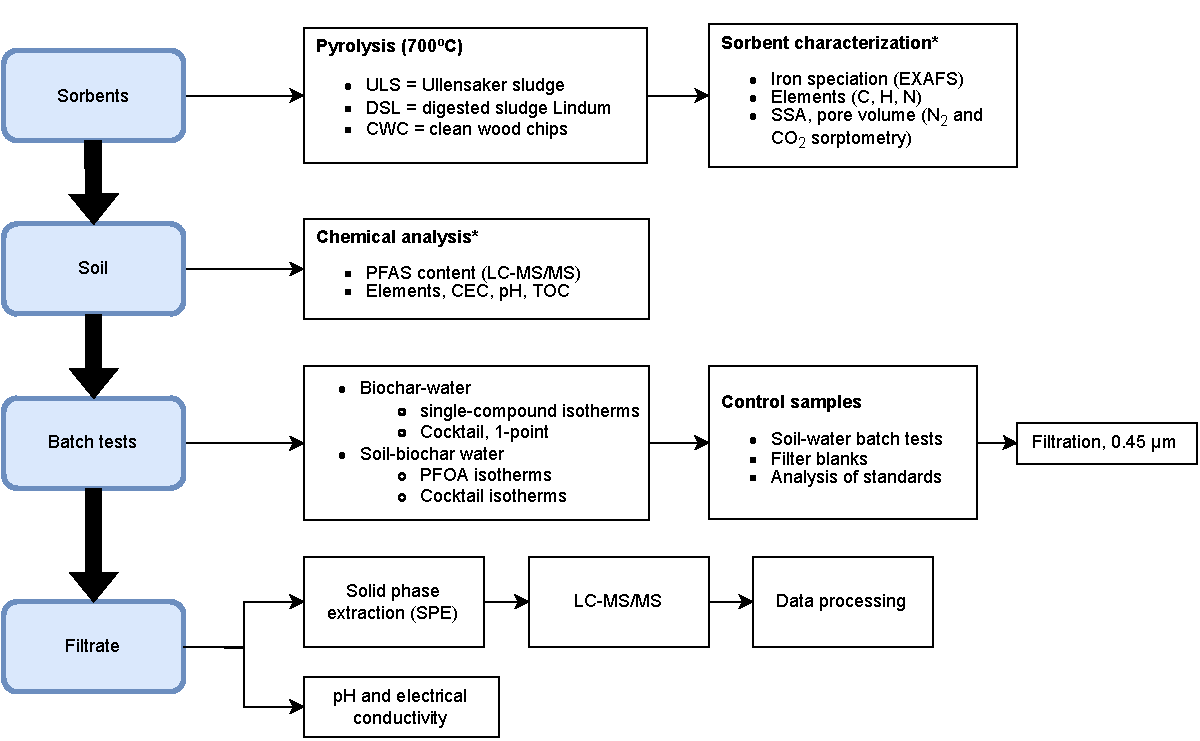
\includegraphics[width=\textwidth]{Diagrams/Methods-General_overview_methods.pdf}
    \caption{Overview of the methods conducted for this thesis. * = analyses conducted by commercial laboratories or that were delegated to project partners.}
    \label{fig:methodoverview}
\end{figure}

\section{Biochar sorbents}
\subsection{Pyrolysis}
CWC, ULS, and DSL biochars were produced by slow pyrolysis at 700 \textdegree C using ETIA technology by Biogreen\textsuperscript{\textcopyright} at Lindum AS (Drammen, Norway). \cref{tab:sorbents} summarizes the variables for pyrolysis of each biochar. The three biochars were produced as part of a larger study on the life cycle of waste based sorbents, and were given as biochar samples for the sorption experiments conducted for this thesis. The pyrolysis chamber was first electrically heated to stable pyrolysis temperature. Feedstock pellets were added to a feeding container where a heated rotating screw (Spirajoule\textsuperscript{\textregistered}) led the feedstock through the pyrolysis chamber for the wanted residence time. The biochar was then transported to an external collection container where it was dispensed into sampling bags \cref{fig:biocharCollection}. \cref{fig:pellets} shows the pellets before and after pyrolysis. 

\begin{table}
\centering
\caption{Pyrolysis temperature (PT), residence time (RT) and feedstock for the biochars used in the sorption experiments.}
\label{tab:sorbents}
\begin{tabular}{llll}
\toprule
Biochar   & PT & RT & Feedstock \\
sorbent & (\textdegree C) & (min) \\
\midrule
CWC  & 700 & 20 & clean wood chips  \\
ULS & 700 & 40  & Ullensaker sludge\\
DSL & 700 & 20 & Digested sludge Lindum \\
\bottomrule
\end{tabular}
\end{table}

\begin{figure}
    \centering
    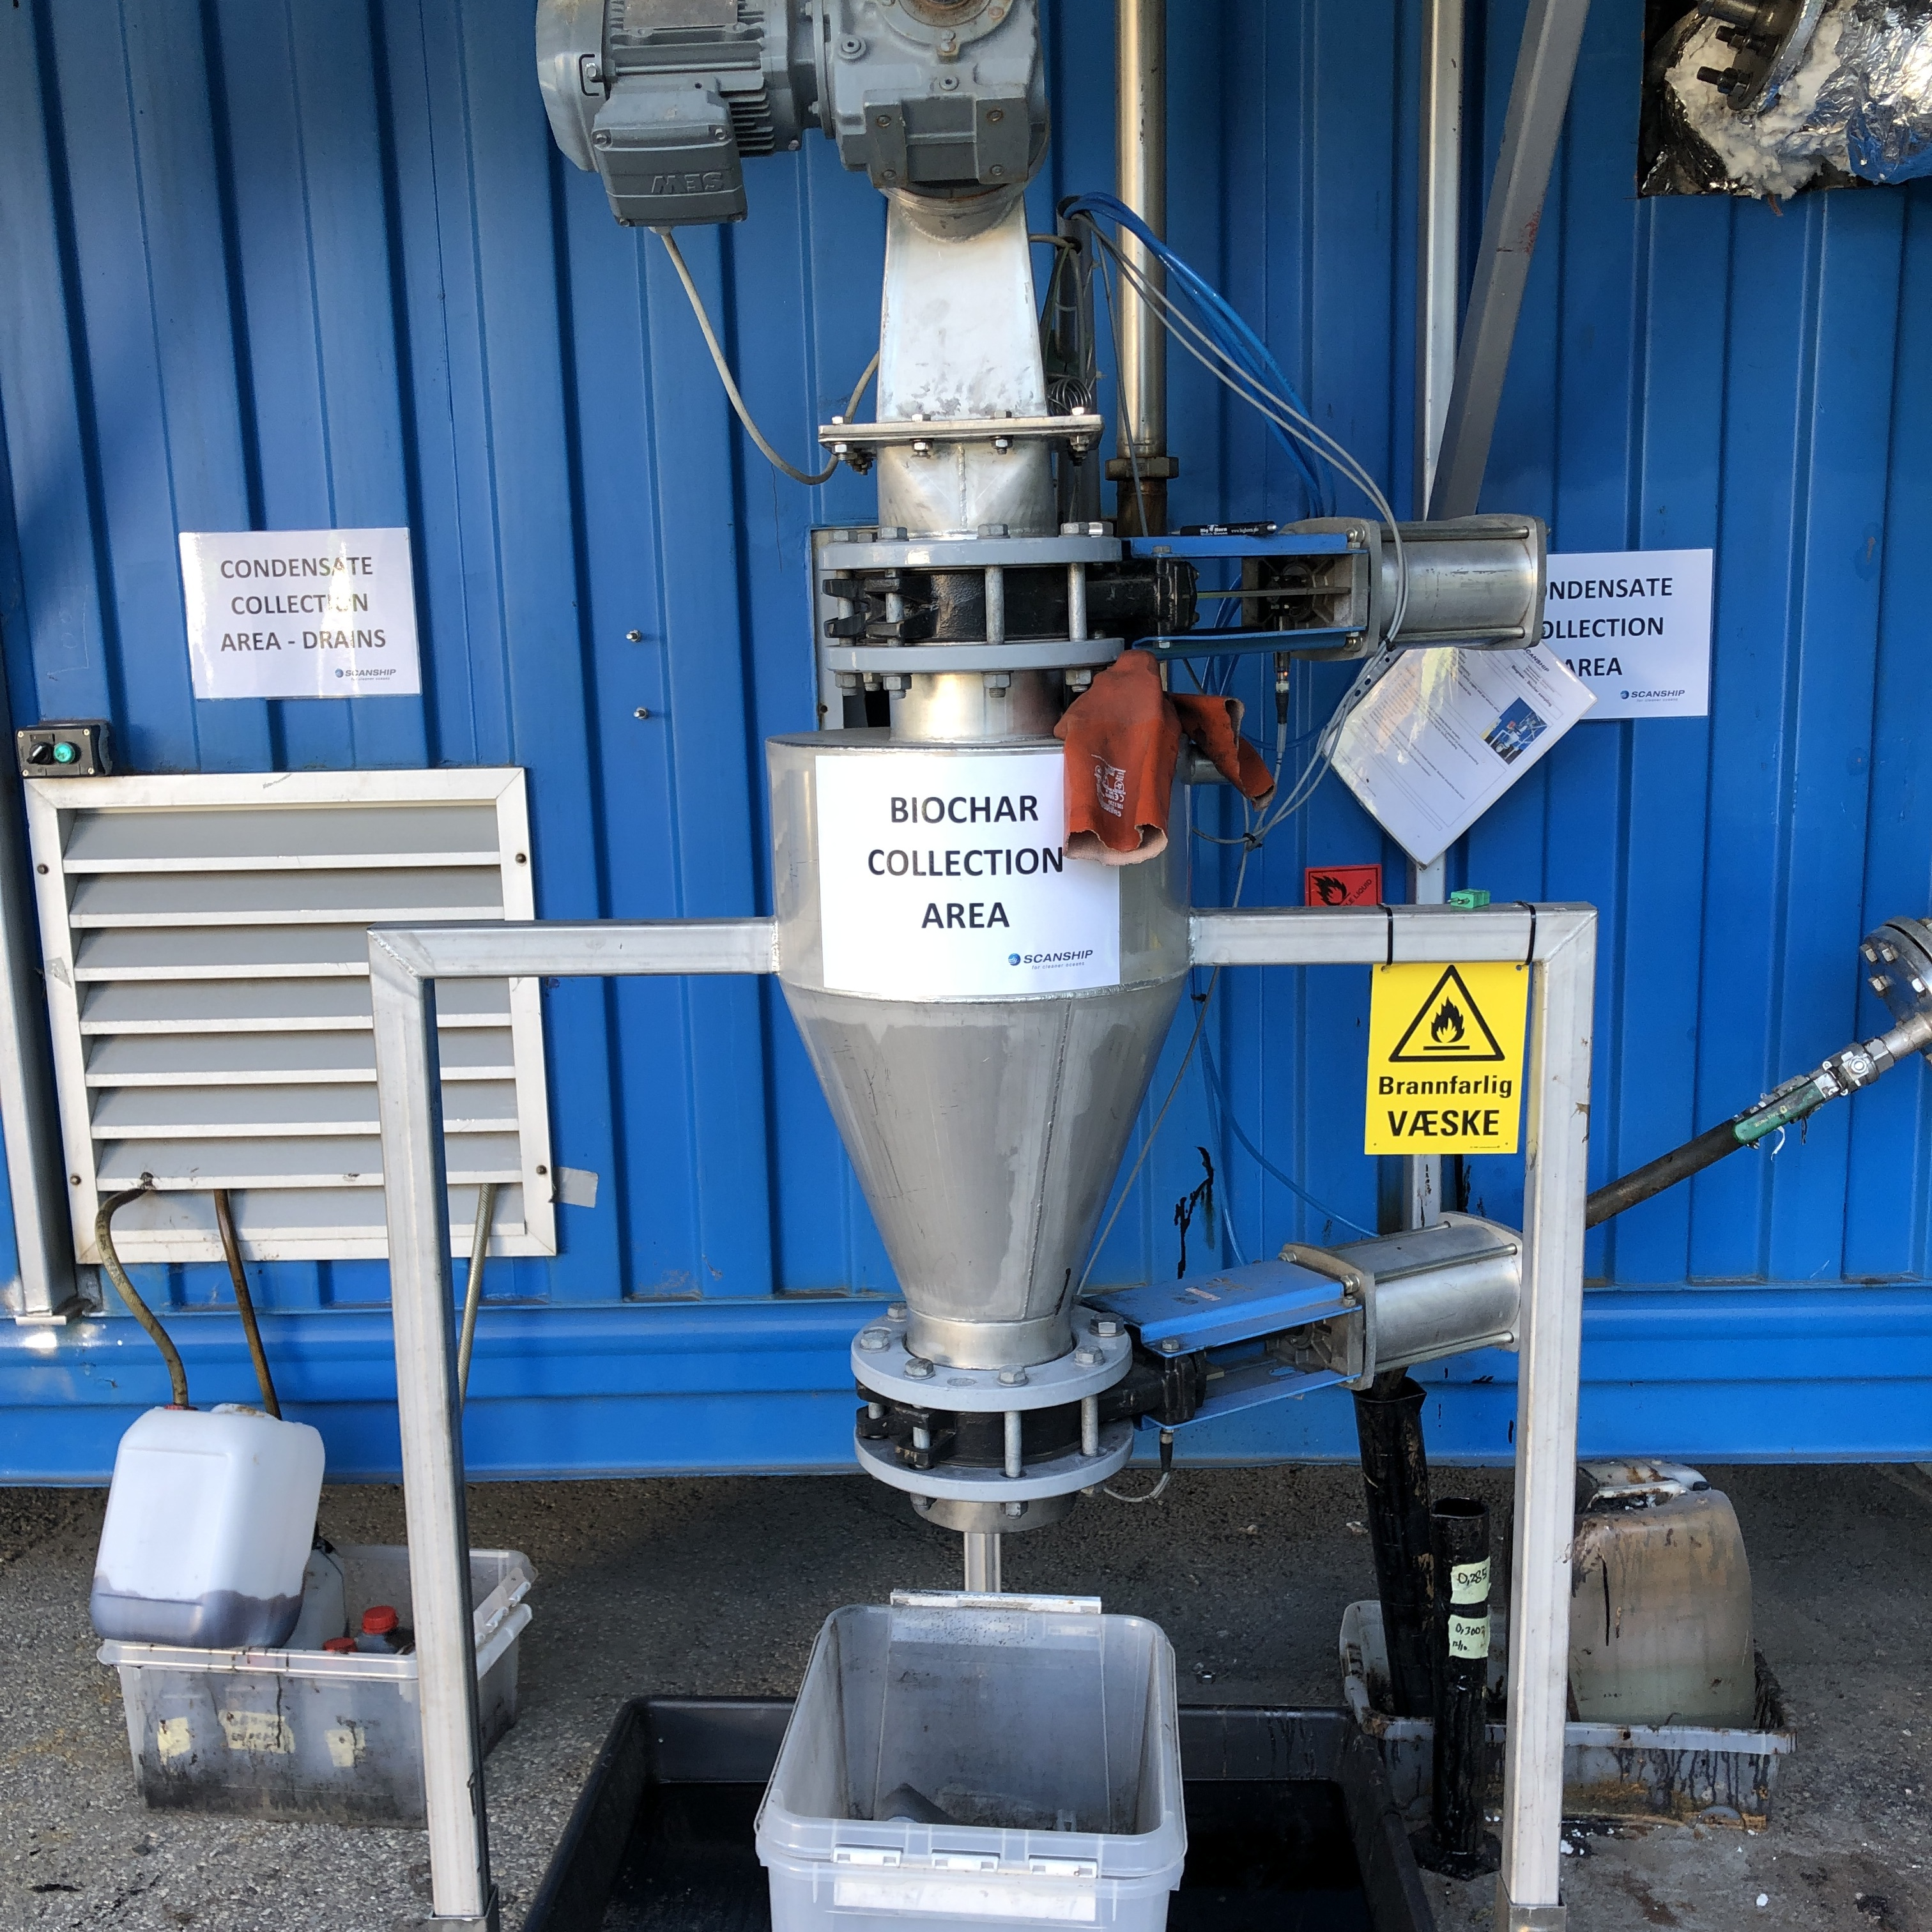
\includegraphics[width=0.6\linewidth,scale=0.6]{Bilder/Pyrolysis/BiocharCollection.jpg}
    \caption{Biochar collection area.}
    \label{fig:biocharCollection}
\end{figure}

\begin{figure}
    \centering
    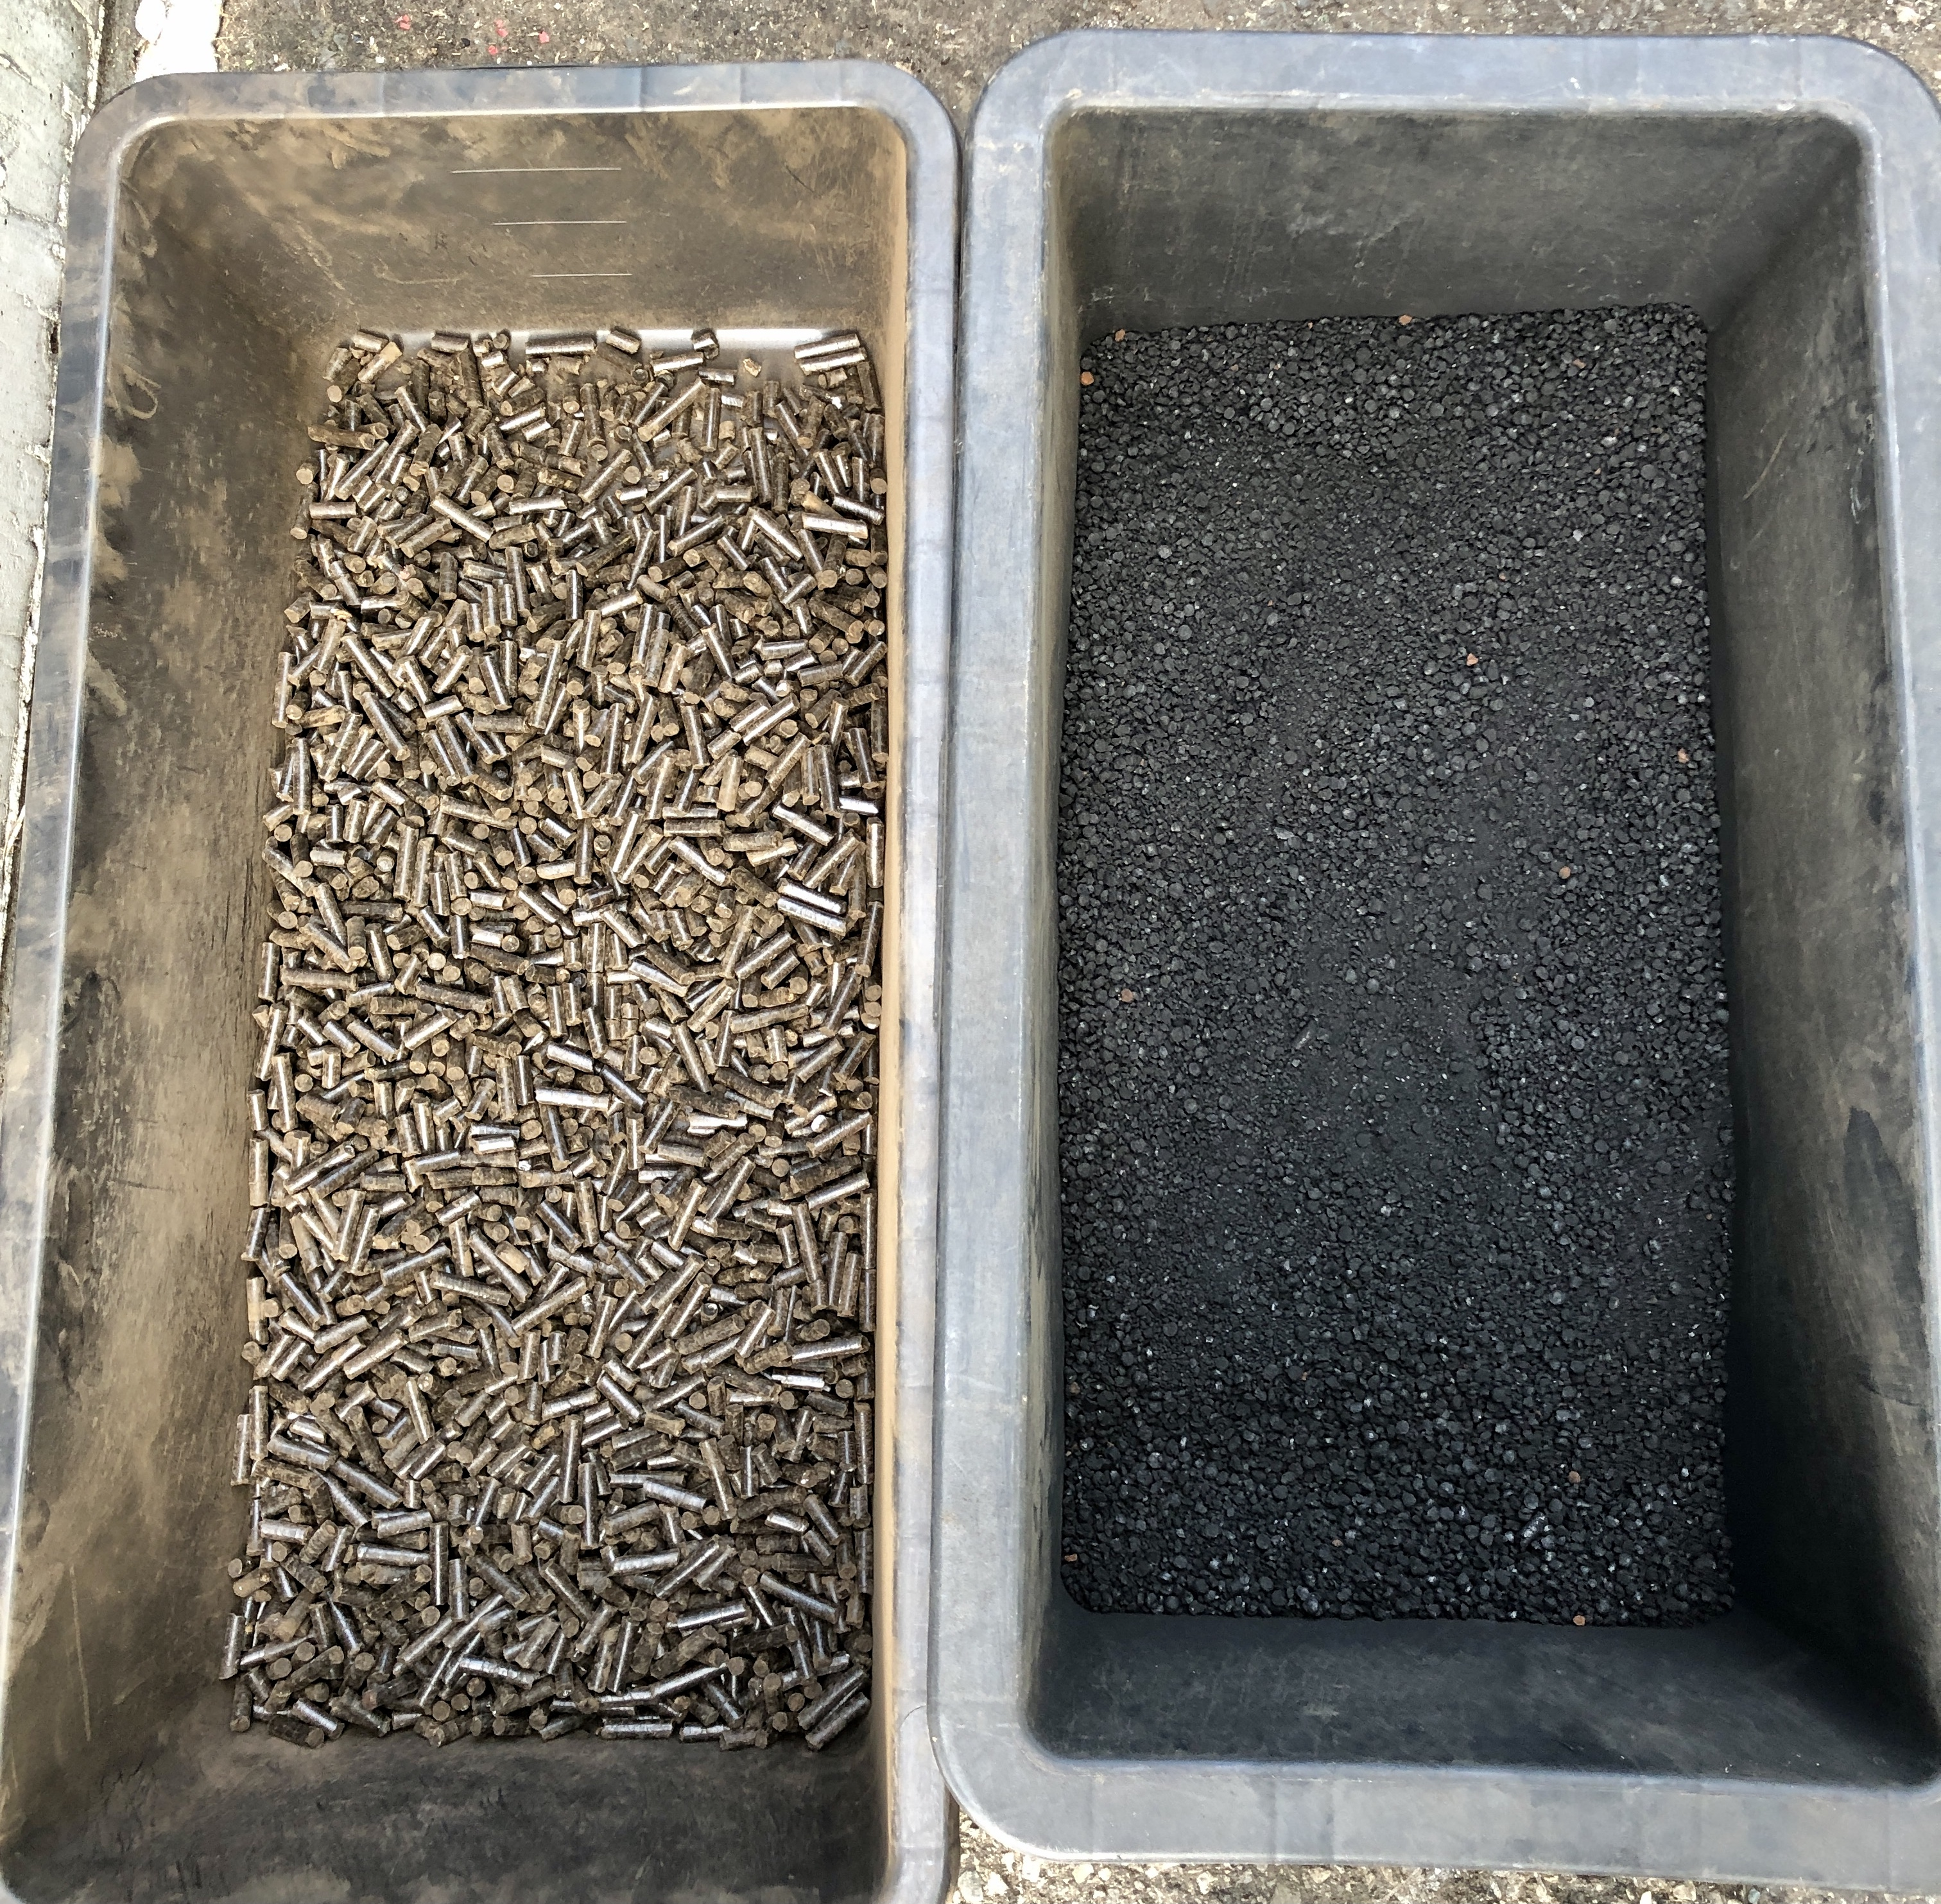
\includegraphics[width=0.6\linewidth,scale=0.6]{Bilder/Pyrolysis/Pellets.png}
    \caption{DSL feedstock pellets (left) and pyrolyzed pellets/biochar (right).}
    \label{fig:pellets}
\end{figure}

Syn-gas from pyrolysis was led through a condensing pipe that condenses into bio-oil at two points depending on boiling point. Syn-gas that does not condense at this point was led into a combustion chamber where a steady inflow of propane ensured a clean burning process of the remaining compounds.

\subsection{Biochar characterization}

\subsubsection{Surface area and pore volume}
Total specific surface area (SA) and pore volume (PV) were determined by nitrogen ($\mathrm{N_2}$) and carbon dioxide ($\mathrm{CO_2}$) gas sorptiometry conducted by research partners at the Particle Engineering Research Center, University of Florida (Gainesville, USA) with a Quantachrome Autosorb 1 surface area analyzer according to the methods described by \cite{kwon2005}. $\mathrm{N_2}$ sorptiometry was performed at the boiling point for liquid nitrogen (-195.8 \textdegree C). Due to slow diffusion at this low temperature, $\mathrm{N_2}$ cannot enter the smallest pores $<$1.5 nm and thus, sorption of $\mathrm{N_2}$ represents the largest pores of \textgreater 1.5 nm. $\mathrm{CO_2}$ sorptiometry was performed at 0 \textdegree C, enabling the gas to diffuse into smaller nanopores between 0.4-1.5 nm. $\mathrm{N_2}$ SA was interpreted using both Brunauer, Emmett and Teller (BET) and density functional theory (DFT). $\mathrm{N_2}$ PV was interpreted with Barret-Joyner-Halenda (BJH) and DFT. $\mathrm{CO_2}$ SA and PV were interpreted with DFT. 

\subsubsection{Element analysis}
Elemental composition (total C, H and N) was performed by project partners by $\mathrm{NO_3}$ digestion and quantified with a Leco CHN-1000 from Leco Corporations (Sollentuna, Sweden), according to DIN 51732.  

\subsubsection{Iron speciation}
Iron speciation of DSL and ULS were analyzed by Fe K-edge X-ray absorption fine structures (EXAFS) at the synchrotron SOLEIL (Gif-sur-Yvette, France) (beamline SAMBA) by a project partner at NGI, with practical contributions from the author of this thesis. To prepare the biochars for analysis, each sample ($\sim$50 mg) was crushed in a mortar to a fine powder (250 \textmu m). The samples were mixed with boron nitride (BN, 300 mg) to a homogeneous powder and pelletized. The BN matrix is used for sample dilution because it absorbs very little of the photon beam at the Fe K-edge. The resulting biochar pellet was analyzed by X-ray absorption spectroscopy.

The overall principle of EXAFS is to determine structural composition of a sample by examining its X-ray absorption spectrum. This plots absorbance, $\mu x$, as a function of photon energy, $eV$ \citep{vlaica2004exafs}. The sample was submitted to an X-ray beam where a spectrophotometer measures the beam's intensity as it passes through the sample. The difference in intensity between before and after the sample is translated into an absorption coefficient, following Beer-Lambert's Law: 

\begin{equation}\label{eq:absorbance}
    \mu x = log \frac{I}{I_0}
\end{equation}

where $\mu x$ is a dimensionless absorbance coefficient ($AU$), $I$ is the transmitted light intensity and $I_0$ is the incident light intensity. The energy of the photon beam is determined by the angle of a crystal monochromator. The angle of the crystal monochromator is tuned so that the sample is bombarded by a range of photon energies in which the absorption edges of the target element lie within \citep{vlaica2004exafs}. An adsorption K-edge occurs when the transmitted photon energy equals the energy required to excite a core electron which is observed as a vertical jump (K) in $\mu x$ on the spectrum \citep{vlaica2004exafs}. The neighboring elements are interfering with the photon wave that translates into oscillations on the absorption spectrum following the absorption edge. Each element has a different retro diffusion coefficient. Therefore, the frequency and amplitude of oscillations in the absorption spectrum are (partially) determined by the type and number of neighboring atoms. The absorption edge energy and oscillations thus contain information on the valency of the element, as well as the number and type of neighboring atoms, i.e., the element speciation. Fe(II) species will have their K edge at a lower energy than Fe(III) species because a higher photon energy is required to excite an electron from the more electronegative Fe(III). In addition, the oscillations will differ depending on the Fe mineral. The different iron species present in the sample can be derived by interpreting the X-ray absorption spectrum.

%%%%%%%%%%%%%%%%%%%%%%%%%%%%%%%%%%%%%%%%%%%%%%%%%%%%%%%%%%%%%%%%%%%%%%%%%%%%%%%%%%%%%%%%%%%%%%%%%%%%%%%%%%%%%%%

\section{Sorption experiments}
\subsection{Experiment preparations}
\subsubsection{Biochar}
A sub-sample (100 g) was taken by random grab sampling from the bulk volume of the biochar produced during pyrolysis. The biochars were crushed using a ball mill (Retsch ISO 9001) with five balls at 50 rpm for 5 minutes, then sieved into fine-powdered biochar (D \textless 1 mm) and transferred to LDPE zipper bags for storage (4 \textdegree C). 

\subsubsection{PFCA sorbates}\label{sec:PFCAanalytic}
In this thesis, six perfluorinated carboxylic acids (PFCAs) were selected as target compounds for the batch test experiments. These were: PFPeA, PFHxA, PFHpA, PFOA, PFNA, PFDA, with perfluorinated carbon units 4-9 respectively (Full names in \cref{tab:PFCAs}). 10 mL stock solutions were prepared for each PFCA by weighing the pure compound salt/liquid (\cref{tab:PFCAs}) on an analytical scale and dissolving them in methanol in volumetric flasks. Additional safety precautions were taken during this procedure by using double Latex gloves. 

Two spiking standards at high (STD1) and low (STD2) concentrations were prepared from the stock solution used for spiking the batch tests at various concentrations (\cref{apptab:standards}). The working standards were analyzed using LC-MS/MS of a twice diluted standard at an optimum concentration for the instrument calibration curve (10-20 \textmu g L\textsuperscript{-1}). All further calculations of spike dilutions were corrected with the help of the measured standard concentrations. See \cref{appSec:IsothermSetup} for expected vs. analytical concentrations. 

\begin{table}
\centering
\caption{PFAS compounds investigated in this study. PFCs correspond to the number of perfluorinated carbon units in the chain. Note: PFCAs appear in dissociated form at environmentally relevant pH's due to low $pK_a$'s.}
\adjustbox{max width=\textwidth}{
\label{tab:PFCAs}
\begin{tabular}{@{}lcccclc@{}}
\toprule
\multicolumn{1}{c}{Chemical} & Acronym & Short & CAS number & Molecular structure & Stock form & Purity \\ \midrule
& & & & & &\\
\smash{\raisebox{4ex}{Perfluoropentanoic acid}}  & \smash{\raisebox{4ex}{PFPeA}} & \smash{\raisebox{4ex}{C5}} & \smash{\raisebox{4ex}{2706-90-3}} & \chemfig[atom style={scale=0.4}]{O=[:90](-[:30,,,1]OH)-[:150](-[:112.5]F)(-[:67.5]F)-[:210](-[:292.5]F)(-[:247.5]F)-[:150](-[:112.5]F)(-[:67.5]F)-[:210](-[:270]F)(-[:150]F)-[:210]F} & \smash{\raisebox{4ex}{liquid}} & \smash{\raisebox{4ex}{\textgreater 97 \%}} \\
& & & & & &\\
\smash{\raisebox{4ex}{Perfluorohexanoic acid}} & \smash{\raisebox{4ex}{PFHxA}}  & \smash{\raisebox{4ex}{C6}} & \smash{\raisebox{4ex}{307-24-4}} & \chemfig[atom style={scale=0.4}]{O=[:90](-[:30,,,1]OH)-[:150](-[:112.5]F)(-[:67.5]F)-[:210](-[:292.5]F)(-[:247.5]F)-[:150](-[:112.5]F)(-[:67.5]F)-[:210](-[:292.5]F)(-[:247.5]F)-[:150](-[:210]F)(-[:150]F)-[:90]F} & \smash{\raisebox{4ex}{liquid}} & \smash{\raisebox{4ex}{\textgreater 97 \%}} \\
& & & & & &\\
\smash{\raisebox{4ex}{Perfluoroheptanoic acid}} & \smash{\raisebox{4ex}{PFHpA}} & \smash{\raisebox{4ex}{C7}} & \smash{\raisebox{4ex}{375-85-9}} & \chemfig[atom style={scale=0.4}]{O=[:90](-[:30,,,1]OH)-[:150](-[:67.5]F)(-[:112.5]F)-[:210](-[:247.5]F)(-[:292.5]F)-[:150](-[:67.5]F)(-[:112.5]F)-[:210](-[:247.5]F)(-[:292.5]F)-[:150](-[:67.5]F)(-[:112.5]F)-[:210](-[:150]F)(-[:210]F)-[:270]F} & \smash{\raisebox{4ex}{crystalline}} & \smash{\raisebox{4ex}{\textgreater 99 \%}} \\
& & & & & &\\
\smash{\raisebox{4ex}{Perfluorooctanoic acid}} & \smash{\raisebox{4ex}{PFOA}}  & \smash{\raisebox{4ex}{C8}} & \smash{\raisebox{4ex}{335-76-2}}  & \chemfig[atom style={scale=0.4}]{O=[:90](-[:30,,,1]OH)-[:150](-[:67.5]F)(-[:112.5]F)-[:210](-[:247.5]F)(-[:292.5]F)-[:150](-[:67.5]F)(-[:112.5]F)-[:210](-[:247.5]F)(-[:292.5]F)-[:150](-[:67.5]F)(-[:112.5]F)-[:210](-[:247.5]F)(-[:292.5]F)-[:150](-[:90]F)(-[:150]F)-[:210]F} & \smash{\raisebox{4ex}{powder}} & \smash{\raisebox{4ex}{\textgreater 95 \%}} \\
& & & & & &\\
\smash{\raisebox{4ex}{Perfluorononaoic acid}}  & \smash{\raisebox{4ex}{PFNA}} & \smash{\raisebox{4ex}{C9}} & \smash{\raisebox{4ex}{375-95-1}} & \chemfig[atom style={scale=0.4}]{O=[:90](-[:30,,,1]OH)-[:150](-[:112.5]F)(-[:67.5]F)-[:210](-[:292.5]F)(-[:247.5]F)-[:150](-[:112.5]F)(-[:67.5]F)-[:210](-[:292.5])(-[:247.5]F)-[:150](-[:112.5]F)(-[:67.5]F)-[:210](-[:292.5]F)(-[:247.5]F)-[:150](-[:112.5]F)(-[:67.5]F)-[:210](-[:270]F)(-[:210]F)-[:150]F} & \smash{\raisebox{4ex}{crystalline}} & \smash{\raisebox{4ex}{\textgreater 97 \%}} \\
& & & & & &\\
\smash{\raisebox{4ex}{Perfluorodecanoic acid}}  & \smash{\raisebox{4ex}{PFDA}}  & \smash{\raisebox{4ex}{C10}} & \smash{\raisebox{4ex}{335-67-1}} & \chemfig[atom style={scale=0.4}]{O=[:90](-[:30,,,1]OH)-[:150](-[:112.5]F)(-[:67.5]F)-[:210](-[:292.5]F)(-[:247.5]F)-[:150](-[:112.5]F)(-[:67.5]F)-[:210](-[:292.5]F)(-[:247.5]F)-[:150](-[:112.5]F)(-[:67.5]F)-[:210](-[:292.5]F)(-[:247.5]F)-[:150](-[:112.5]F)(-[:67.5]F)-[:210](-[:292.5]F)(-[:247.5]F)-[:150](-[:210]F)(-[:150]F)-[:90]F} & \smash{\raisebox{4ex}{flakes}} & \smash{\raisebox{4ex}{\textgreater 98\%}} \\
& & & & & &\\ \bottomrule
\end{tabular}}
\end{table}

\subsubsection{Spike concentrations}
The goal when designing the sorption isotherm experiments was to represent sorption to each biochar sample across both the linear and non-linear regions. To achieve detectable equilibrium in aqueous concentrations ($C_w$), determination of appropriate spike concentrations was based on several factors: 1) biochar-water partition coefficients ($K_{BC}$) for the corresponding PFCAs obtained from literature \cite{Xiao2017} \cref{apptab:Kbc}, 2) biochar dose, 3) LOQ of the analytical method (\cref{apptab:LOQ}), and 4) available volumes of pipette tips. The relationship between $K_{BC}~\mathrm{(L~kg^{-1})}$, the sorbed concentration, $C_s~\mathrm{(\mu g~kg^{-1})}$, and the freely dissolved aqueous concentration, $C_w~\mathrm{(\mu g~L^{-1})}$, is expressed as:

\begin{align}
    \label{eq:Kbc1}
    K_{BC} = \frac{C_s}{C_w}
\end{align}

and was used to estimate the expected $C_w$. By rearranging \cref{eq:Kbc1}, $C_w$ can be expressed as a function of the mass PFCA spiked ($m_{TA}$), the estimated $K_d$, the biochar dose ($m_{BC}$), and sample water volume ($V_w$):

\begin{align}
    \label{eq:Cw2}
    C_w=\frac{\frac{m_{PFAS}}{\left (\frac{m_{BC}\times K_{BC}}{V_w}\right)+1}}{V_w}
\end{align}

The lowest spike concentration for each isotherm was decided to be two times the method LOQ to account for uncertainties in $C_w$-estimation. The remaining points were spread evenly over a $10^4$ concentration interval. Two preliminary batch tests were prepared to check how well the preliminary estimations matched the sorption affinities of the present biochar samples (more information in \cref{appSec:IsothermSetup}).

\subsubsection{Soil}
Soil used for the attenuation sorption tests in the presence of soil was an unaged sandy soil obtained from a remote field area 17 km from Uppsala, Sweden (59.733 N, 17.667 E). The soil carbon content was determined through dry combustion according to ISO10694 (1995) using an elemental analyzer for macro samples (TruMac\textregistered CN, Leco corp, St. Joseph, MI, USA), performed by research partners at the Swedish University of Agricultural Sciences (SLU), Uppsala, Sweden. The soil was classified as a fine sand (0.1 to 0.3 mm) with 1.3 \% TOC (pH 5.38 $\pm$ 0.02, CEC 2.63 $\pm$ 0.06 meqv 100 g\textsuperscript{-1}). Total element concentrations and exchangeable ion concentrations are in \cref{appSec:elements}, \cref{apptab:soil}. Soil extraction showed no native PFCAs present.

The soil was dried at 100 \textdegree C for 24 h and crushed and sieved to \textless 2 mm.  A project partner at NTNU, Trondheim, Norway screened the soil for PFAS using a methanol extraction, solid phase extraction (SPE) and quantification by liquid chromatography-tandem mass spectrometry (LC-MS/MS). 

\subsection{Batch tests\label{sec:S-BC}}
Batch tests were prepared with a liquid to solid mass ratio (L/S) of 500 for biochar, and an L/S of 10 for soil amended with 2\% biochar in accordance with CEN EN 12457 with modifications described in \citep{Hale2017fire, kupryianchyk2016biochar}. An overview of the experimental setup for the batch tests is given in \cref{fig:batchtests_flowchart}, and an illustration of the batch test experiment procedure is in \cref{fig:batchtest_setup}.

All samples were prepared in 50 mL polypropylene (PP) centrifuge tubes that were rinsed three times with 50\% MeOH to extract any potential PFAS contamination prior to sample preparation. 100$\pm$4 mg biochar or 5$\pm$0.005 g soil and 100$\pm$4 mg biochar were added to the sample tubes and spiked with single PFCA compounds and PFCA cocktail at the concentrations specified in \cref{tab:spikeConcentrations}, then filled with Milli-Q water to final sample volumes of 50 mL. Water volume was first measured by pouring to the 50 mL mark, but after the first 120 samples, the remaining samples were weighed to achieve greater accuracy. Cocktail samples were spiked with the same relative amounts of each PFCA as the single-spike samples at SC10 (SC10-MIX). The concentrations spiked were compared to literature values for the critical micelle concentrations (CMC) of the different PFCAs and were not an issue for the concentration range considered \citep{bhhatarai2011,ding2013physicochemical}. the samples were assured to contain $<$10\% MeOH, which is the upper limit for which methanol does not influence sorption \citep{arvaniti2014}.

Batch tests were shaken end-over-end (9 rpm) and/or agitated on a shaking table (160 rpm) at room temperature (23\textdegree C) for at least 14 days in order to reach equilibrium \citep{higgins2006sorption}. The samples were filtered through a 0.45 \textmu m Minisart\textsuperscript{\textregistered} regenerated cellulose syringe filter into new \acrshort{PP} tubes according to methods described in \cite{Sorengard2019}. Prior to filtration, the samples containing soil were centrifuged to remove as many particles from suspension as possible. However, filtration still required frequent filter change due to clogging (up to three times per sample). Loss of biochar that adhered to the walls of the syringe was quantified in the event that a full mass balance was required for analysis of PFCA partitioning \cref{appSec:misclab}. However, a 100\% mass balance was assumed when calculating partitioning between sorbent and water. The calculation was done by subtracting the initial spike concentration from the measured filtrate concentration.

\section{Soil}\label{sec:Soil}
Before filtration of the batch tests with soil, each sample category (CWC-soil, DSL-soil, ULS-soil and soil only), despite being centrifuged, contained different degrees of suspended particles. This made it difficult to filter the samples that contained the most suspended particles. Filtration led to clogged filters that had to be changed up to three times per sample. The resulting filtrates varied in color \cref{fig:DOC}. These differences can be attributed to different amounts of dissolved organic carbon (\acrshort{DOC}). The sludge biochar-soil samples were more transparent than soil only and soil-CWC. The remarkable difference in DOC is attributed to DOC complexation with inorganic species present in the sludge chars, but not in CWC. Frequently clogged filters likely resulted in reduced filter pore size associated with the fact that some DOC was retained. This may have led to underestimating $C_w$, and thereby overestimating $K_d$ for soil which, in turn, became an issue when deriving $K_F$ for the biochar in these samples using \cref{eq:FreundLinSoil4}. Filter blanks were only prepared for BC-water samples that showed no significant effect (see \cref{apptab:FB}). Hence, the effect of reduced filter size by clogging cannot be quantified. In summary, the results and observations from the BC soil batch tests indicate that sewage sludge biochar binds DOC, and DOC in the filtrate is potentially responsible for an underestimation of $C_w$, and hence, overestimation of $K_{d,s}$. 

\begin{figure}
    \centering
    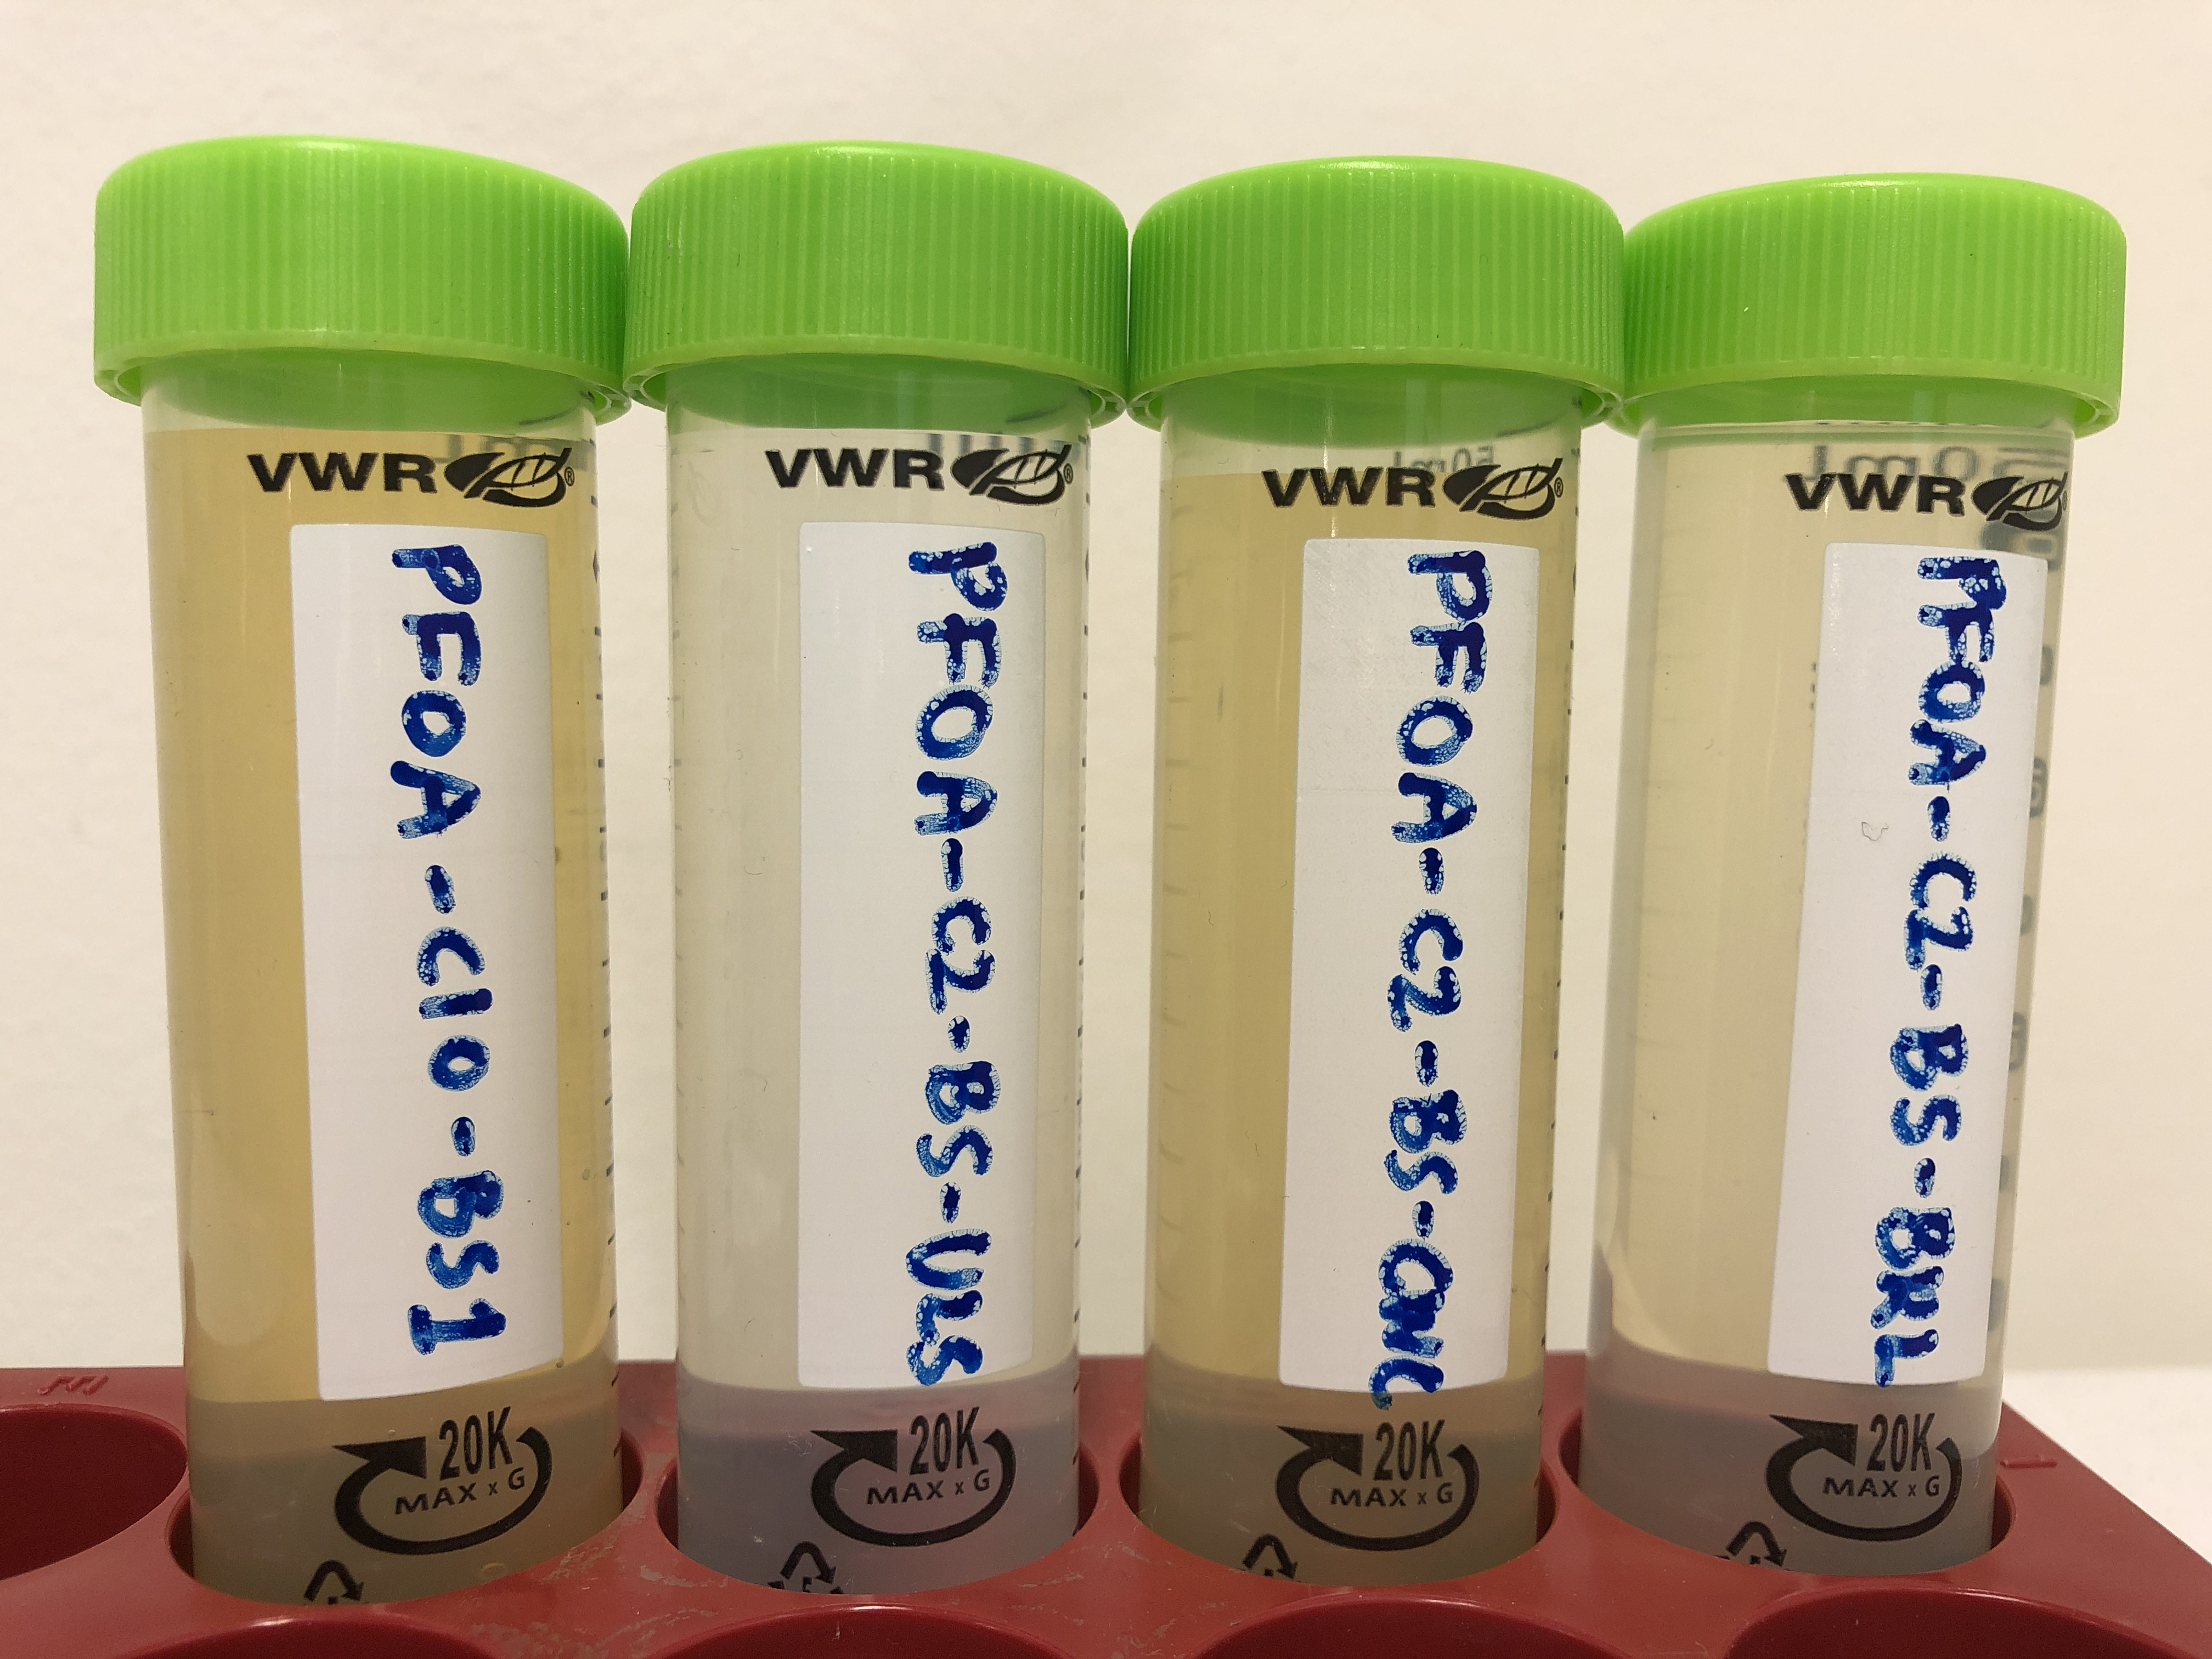
\includegraphics[width=0.7\textwidth]{Bilder/Samples/Filtrate_DOC.JPG}
    \caption{Color of filtrate for each biochar batch test. From left to right: soil only, soil+ULS, soil+CWC, and soil+DSL (BRL = DSL).}
    \label{fig:DOC}
\end{figure}

\begin{figure}
    \centering
    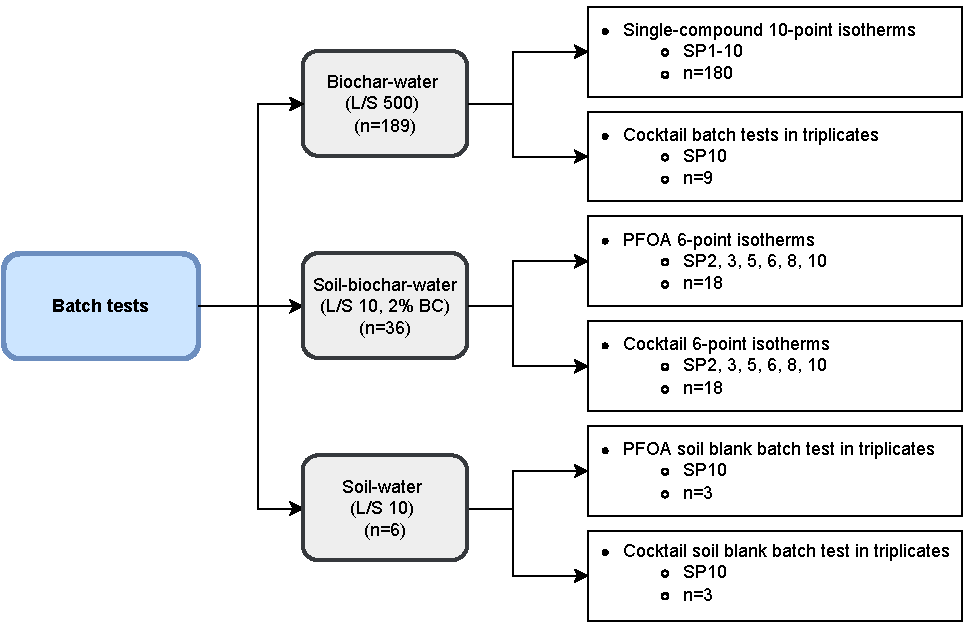
\includegraphics{Diagrams/Methods-Page-9.pdf}
    \caption{Overview of batch test samples for this thesis for the biochar samples (\acrshort{ULS}, \acrshort{DSL}, \acrshort{CWC}) and target compounds (\acrshort{PFPeA}, \acrshort{PFHxA}, \acrshort{PFHpA}, \acrshort{PFOA}, \acrshort{PFNA}, \acrshort{PFDA}). \acrshort{SC} = spike concentration. SC10 = highest spiked concentration.}
    \label{fig:batchtests_flowchart}
\end{figure}

\begin{figure}
    \centering
    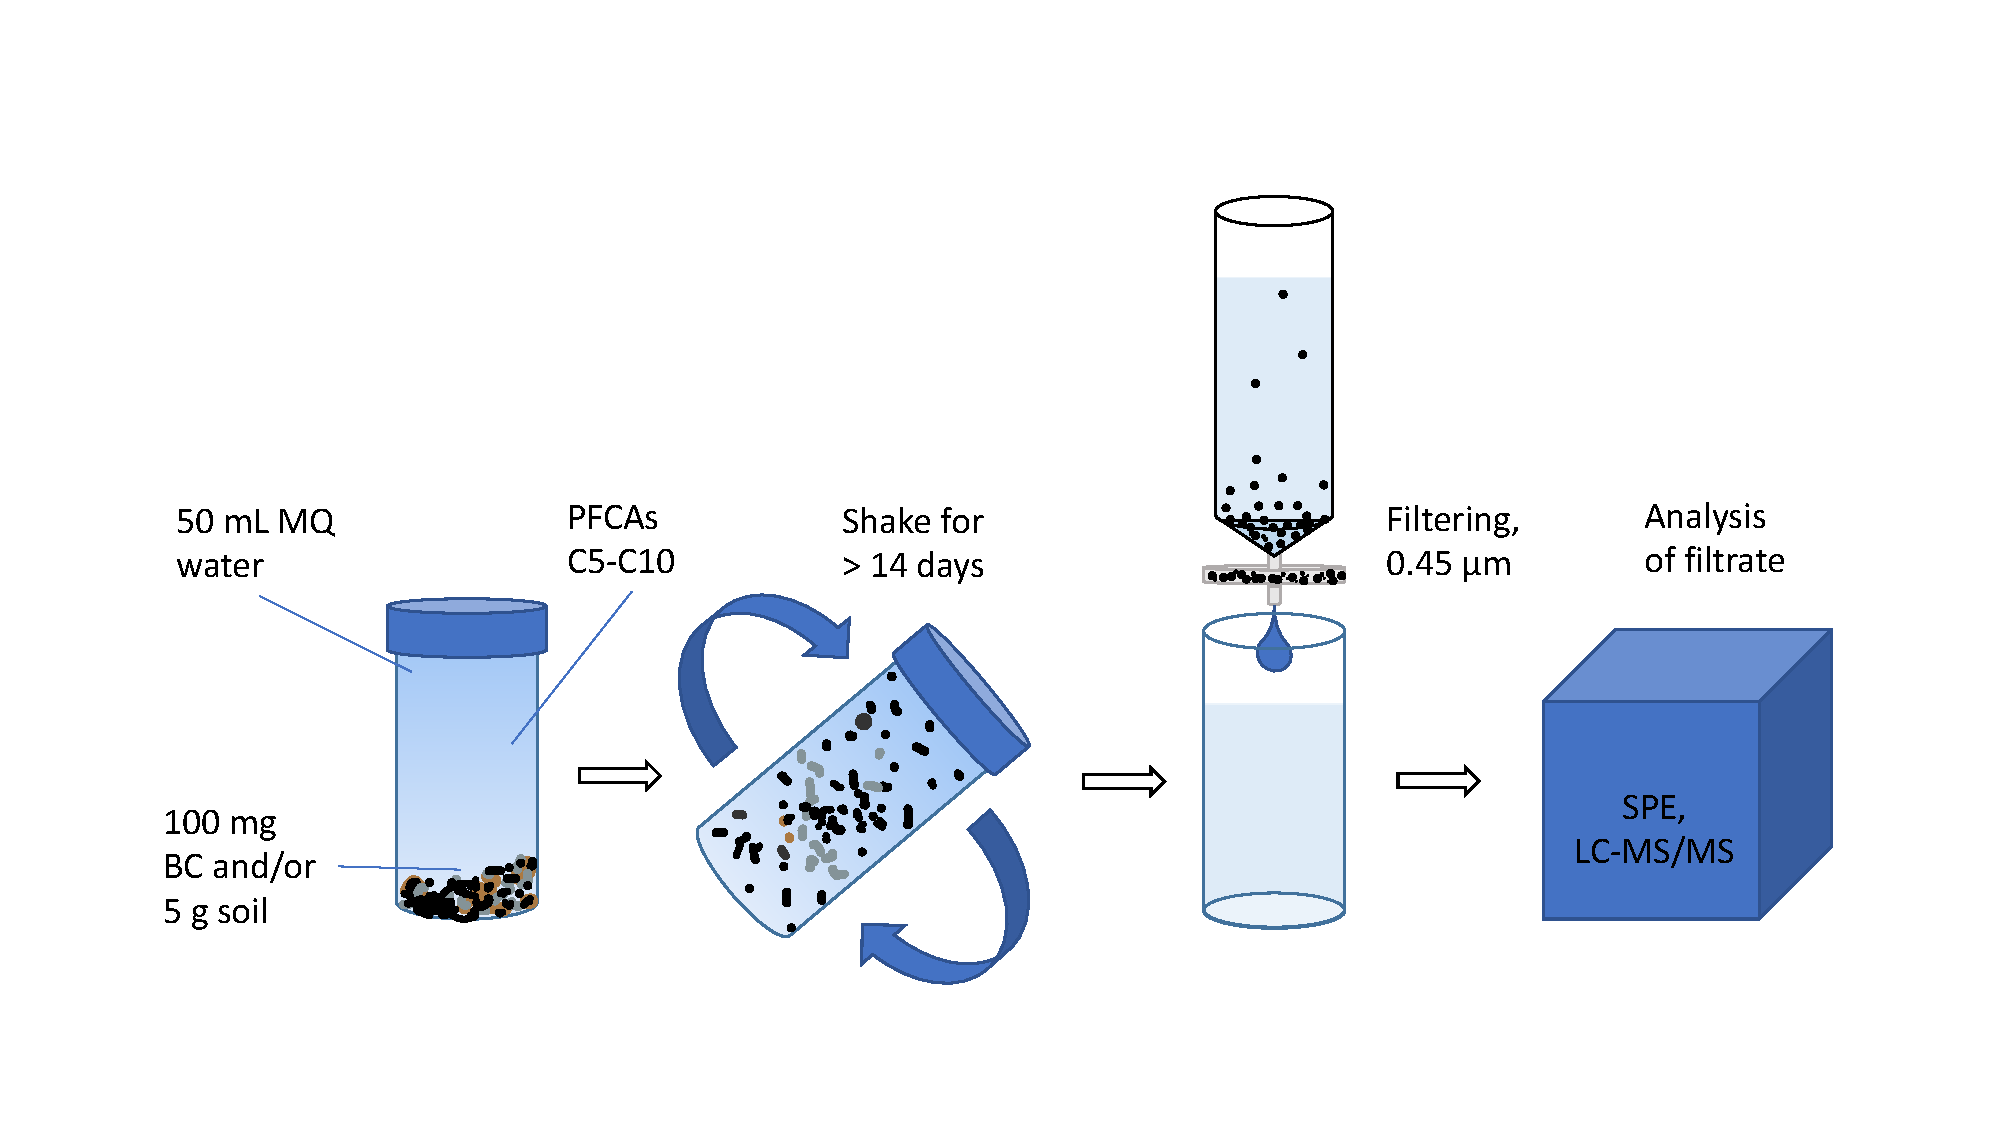
\includegraphics[width=\textwidth]{Diagrams/Batch_test.pdf}
    \caption{Laboratory batch shaking test experimental procedure.}
    \label{fig:batchtest_setup}
\end{figure}

\begin{table}
    \caption{Spike concentrations (SC) in \textmu g L\textsuperscript{-1} used for the batch tests. MIX = cocktail spike concentration for biochar-water batch tests in triplicates, MIX-S = cocktail spike concentration for biochar-soil-water and soil-water batch tests.}
    \label{tab:spikeConcentrations}
    \adjustbox{max width=\textwidth}{%
    \begin{tabular}{lrrrrrrrrrrrr}
    \toprule
    Compound & SC1 & SC2 & SC3 & SC4 & SC5 & SC6 & SC7 & SC8 & SC9 & SC10 & SC10-MIX & SC10-MIX-S \\ \midrule
    PFPeA & 0.019 & 21 & 43 & 64 & 86 & 107 & 128 & 150 & 171 & 191 & 191 & 283\\
    PFHxA & 0.033 & 37 & 73 & 110 & 146 & 184 & 220 & 256 & 292 & 330 & 330 & 836 \\
    PFHpA & 0.012 & 11 & 25 & 38 & 52 & 65 & 79 & 92 & 106 & 117 & 117 & 153\\
    PFOA & 0.195 & 216 & 435 & 651 & 871 & 1 087 & 1 302 & 1 522 & 1 742 & 1 953 & 1 953 & 1 974\\
    PFNA & 0.141 & 156 & 313 & 471 & 625 & 784 & 942 & 1 097 & 1 255 & 1 409 & 1 409 & 2 310\\
    PFDA & 0.383 & 425 & 850 & 1 275 & 1 700 & 2 126 & 2 551 & 2 976 & 3 401 & 3 830 & 3 830 & 5 288\\ \bottomrule
    \end{tabular}}
\end{table}

\subsection{pH and electrical conductivity}
pH and conductivity were measured in a slurry of biochar and water (1:5), with pre-stirring (15 min) and letting the particles settle (\textgreater 24 hrs) before measurement (n=3). 

\subsection{Sample blanks}
To control for potential underestimation of $C_w$, filtration blanks were prepared in triplicate for each PFCA at an optimum concentration range for the instrument (see \cref{sec:PFCAanalytic}) to correct for PFCA-loss to the filter paper. 

%%%%%%%%%%%%%%%%%%%%%%%%%%%%%%%%%%%%%%%%%%%%%%%%%%%%%%%%%%%%%%%%%%%%%%%%%%%%%%%%%%%%%%%%%%%%%%%%%%%%%%%%%%%%%%%%%%%%%%%%%%%%

\section{Instrumental analysis} \label{methods:instrAnalysis}
PFCA quantitation in the filtrates was determined by liquid chromatography--tandem mass spectrometry (LC-MS/MS). Reversed-phase solid phase extraction (SPE) was used as sample preparation method. These analyses were conducted at the Institute of Chemistry at NTNU (Trondheim, Norway).

% missing reconstitution step, update diagram
\begin{figure}
    \centering
    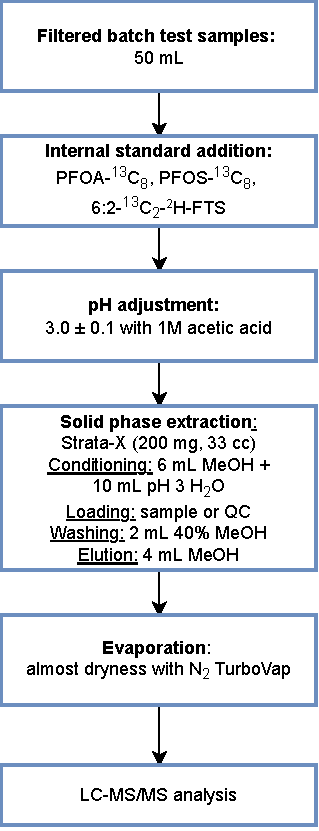
\includegraphics{Diagrams/Methods-Analytical_method.pdf}
    \caption{Schematic diagram of the analytical method applied for the determination of TCs in the batch test filtrates adapted from \cite{arvaniti2012diagram}.}
    \label{fig:analyticalMethod}
\end{figure}

\subsection{SPE}
SPE is a sample preparation method used to extract and concentrate a large-volume sample to produce a solvent extract that can be subjected to analyte quantification by LC-MS/MS. The sample is passed through a cartridge with a porous sorbent polymer serving as the extraction agent that strongly retains polar compounds. The sorbed analytes are then eluted with an appropriate solvent, evaporated, and finally reconstituted to the desired extract volume. All samples are spiked with a mix of internal standards (\acrshort{IS}s) to compensate for variations in extraction percentages and instrumental response by the MS/MS detector \citep{arvaniti2014}. To minimize risk of contamination during laboratory work, working benches were cleaned with acetone and covered with aluminum foil. Sterilized PP tubes were used during all steps of the protocol.

Strata-X\textsuperscript{\textregistered} 200 mg/6mL cartridges, supplied by Phenomenex, were used for \acrshort{SPE} of the target compounds in the filtered water samples. The sorbent polymer was a surface modified styrene divinylbenzene (\cref{fig:StatPhase}) with 33 \textmu m average particle diameter and surface area of 800 m\textsuperscript{2} g\textsuperscript{-1}. The internal standards used were \textsuperscript{13}C\textsubscript{8}-perfluorooctanoic acid  (\textsuperscript{13}C\textsubscript{8}-PFOA), \textsuperscript{13}C\textsubscript{8}-potassium perfluorooctanesulfonate (\textsuperscript{13}C\textsubscript{8}-PFOS-K), and 6:2-\textsuperscript{13}C\textsubscript{2}-\textsuperscript{1}H,\textsuperscript{2}H-perfluorooctane sulfonate  (6:2 \textsuperscript{13}C\textsubscript{2}-FTS) where a working standard of the three isotopic PFASs were prepared in methanol at 1 ppm from 50 ppm analytical standard supplied by Sigma Aldrich.

The samples were adjusted to pH $\sim$3 with 800 \textmu L 1 M acetic acid. However, samples containing soil needed at least double this amount added to reach the same pH. pH strips were used to test the pH of five randomly selected samples from each batch of 20. All samples were then spiked with IS. SC1 and SC2 samples were spiked with 10 \textmu L IS, and SC3-SC10 samples were spiked with 20 \textmu L IS. The difference in the amount of IS for the two low-spike samples was due to the fact that a more concentrated extract was needed for these samples  so as to avoid signals below instrumental \acrshort{LOQ}.  For this reason, SC1 and SC2 samples were reduced to 0.5 mL extracts instead of 1 mL as was the case for the rest. The samples were vortexed prior to SPE.

The SPE cartridges were placed in individual slots with LC liners on a \acrshort{TLC} chamber, and conditioned with 6 mL \acrshort{MeOH} and 10 mL pH 3 milli-Q water (acidified by 100\% acetic acid). MeOH was used for wetting to allow the mobile phase to flow into all the pores of the sorbent polymer, in this way ensuring maximum chromatographic retention. Water with a low pH was used to protonate lone pair electrons on the polymer surface in order to maximize hydrophobic interaction with the analytes. The samples were loaded using glass pipettes and allowed to pass through the cartridges by gravity. The flow rate was adjusted by modifying the opening of the LC liners so that the sample exited the cartridge as individual droplets.

After extraction of the samples, the SPE cartridges were washed with 2 mL MeOH:\acrshort{MQ} (40:60, \% v/v) in order to remove any matrix interferences. The cartridges were then dried with a vacuum pump at 20 mmHg until the extraction agent was visible as a dry powder. The analytes were then eluted with 4 mL MeOH into 15 mL PP centrifuge tubes, and concentrated to near $\le$0.5 mL using TurboVap\textsuperscript{\textregistered} at 40 \textdegree C, and nitrogen gas (N\textsubscript{2}) at 5 psi. The samples were reconstituted to 1 mL (0.5 mL for SCs 1 and 2) with MeOH and MQ, ending up at a final solvent ratio of 50:50 \% v/v. The extracts were transferred to LC vials using glass pipettes and stored at -19 \textdegree C until analysis.

\begin{figure}
    \centering
    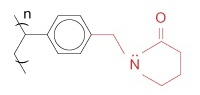
\includegraphics{Bilder/SPE_LCMS/mg_spe_strata-x.jpg}
    \caption{Polymer used as extraction agent in SPE, surface-modified styrene divinylbenzene.}
    \label{fig:StatPhase}
\end{figure}

\subsection{LC-MS/MS}
Liquid chromatography separates compounds in a mixture based on polarity by using a stationary phase that retards hydrophobic compounds while allowing more polar compounds to pass through more quickly along with a polar mobile phase. Using a high voltage, the compounds are then ionized into fragment ions which are detected by a mass spectrometer that determines the mass of the transitions. In the present work, quantification of PFAS was determined by \acrshort{LC-MS/MS} using an Acquity UPLC I-Class system connected to a Xevo TQ-S triple quadrupole mass spectrometer equipped with an ESI Z spray, both supplied by Waters (Milford, MA, USA). A Kinetex C18 column (30 x 2.1 mm, 1.3 \textmu m) serially connected to a Phenomenex C18 (2 x 2.1 mm i.d.) security guard (Torrance, CA, USA) was used for chromatographic separation. Mobile phases were A: 2 mM ammonium acetate in MQ water (water phase) and B: pure MeOH (organic phase) that were supplied at a constant flow rate of 250 \textmu L min\textsuperscript{-1} to the LC column, maintained at a temperature of 30 \textdegree C. The sample injection volume was 4 \textmu L. The run time for each sample was 6 minutes, with an initial and final mobile phase gradient of 20:80 (A:B). Analytes were ionized by negative electrospray ionization (\acrshort{ESI}-), and nitrogen was used as a drying gas at the ionization source. Two ion transitions were monitored for each PFCA (\cref{tab:transitions}) within 60 seconds of the expected retention time for the compound. Peak integration was performed automatically by MassLynx software obtaining 12 points per peak, and an average baseline peak width of 5 s. Data from LC-MS/MS was processed in MassLynx version 4.1, while quantification processing was performed with TargetLynx. Each peak was manually reviewed to remove peaks that were likely background noise as well as corrections for inconsistencies in peak base width. Complete instrument programming and parameters are summarized in \cref{appSec:LCMS}.

\begin{table}[tbh]
\centering
\caption{Ion transitions for the target analytes and internal standards in this study.}
\adjustbox{max width=\textwidth}{%
\begin{threeparttable}
\label{tab:transitions}
\begin{tabular}{ccccccl} \toprule
Compound &  Structure & Formula & M & Parent & Cone (V) & Transitions (CE)  \\ \midrule
& & & & & & \\
\multirow{2}{*}{PFPeA} &  \multirow{2}{*}{\chemfig[atom style={scale=0.5}]{O=[:90](-[:30,,,1]OH)-[:150](-[:112.5]F)(-[:67.5]F)-[:210](-[:292.5]F)(-[:247.5]F)-[:150](-[:112.5]F)(-[:67.5]F)-[:210](-[:270]F)(-[:150]F)-[:210]F}} & \multirow{2}{*}{$\mathrm{C_5HF_9O_2}$} & \multirow{2}{*}{264.05} & \multirow{2}{*}{262.97} & \multirow{2}{*}{20} & \multirow{2}{*}{262.97 $\rightarrow$ 219 (8)} \\
& & & & & & \\
& & & & & & \\
 &  &  &  &  &  &    \\
\multirow{2}{*}{PFHxA} &  \multirow{2}{*}{\chemfig[atom style={scale=0.5}]{O=[:90](-[:30,,,1]OH)-[:150](-[:112.5]F)(-[:67.5]F)-[:210](-[:292.5]F)(-[:247.5]F)-[:150](-[:112.5]F)(-[:67.5]F)-[:210](-[:292.5]F)(-[:247.5]F)-[:150](-[:210]F)(-[:150]F)-[:90]F}} & \multirow{2}{*}{$\mathrm{C_6HF_{11}O_2}$} & \multirow{2}{*}{314.05} & \multirow{2}{*}{312.97} & \multirow{2}{*}{10} & 312.97 $\rightarrow$ 118.95 (18) \\
 &  &  &  &  &  &   312.97 $\rightarrow$ 269 (8) \\
 & & & & & & \\
 & & & & & & \\
\multirow{2}{*}{PFHpA} &  \multirow{2}{*}{\chemfig[atom style={scale=0.5}]{O=[:90](-[:30,,,1]OH)-[:150](-[:67.5]F)(-[:112.5]F)-[:210](-[:247.5]F)(-[:292.5]F)-[:150](-[:67.5]F)(-[:112.5]F)-[:210](-[:247.5]F)(-[:292.5]F)-[:150](-[:67.5]F)(-[:112.5]F)-[:210](-[:150]F)(-[:210]F)-[:270]F}} & \multirow{2}{*}{$\mathrm{C_7HF_{13}O_2}$} & \multirow{2}{*}{364} & \multirow{2}{*}{362.96} & \multirow{2}{*}{6} & 362.96 $\rightarrow$ 119.00 (22) \\
 &  &  &  &  &  &   362.96 $\rightarrow$ 168.97 (18) \\
 & & & & & & \\
 & & & & & & \\
\multirow{2}{*}{PFOA} &  \multirow{2}{*}{\chemfig[atom style={scale=0.5}]{O=[:90](-[:30,,,1]OH)-[:150](-[:67.5]F)(-[:112.5]F)-[:210](-[:247.5]F)(-[:292.5]F)-[:150](-[:67.5]F)(-[:112.5]F)-[:210](-[:247.5]F)(-[:292.5]F)-[:150](-[:67.5]F)(-[:112.5]F)-[:210](-[:247.5]F)(-[:292.5]F)-[:150](-[:90]F)(-[:150]F)-[:210]F}} & \multirow{2}{*}{$\mathrm{C_8HF_{15}O_2}$} & \multirow{2}{*}{414.07} & \multirow{2}{*}{412.97} & \multirow{2}{*}{20} & 412.97 $\rightarrow$ 168.90 (18) \\
 &  &  &  &  &    & 412.97 $\rightarrow$ 369.00 (8) \\
 & & & & & & \\
 & & & & & & \\
\multirow{2}{*}{PFNA} &  \multirow{2}{*}{\chemfig[atom style={scale=0.5}]{O=[:90](-[:30,,,1]OH)-[:150](-[:112.5]F)(-[:67.5]F)-[:210](-[:292.5]F)(-[:247.5]F)-[:150](-[:112.5]F)(-[:67.5]F)-[:210](-[:292.5])(-[:247.5]F)-[:150](-[:112.5]F)(-[:67.5]F)-[:210](-[:292.5]F)(-[:247.5]F)-[:150](-[:112.5]F)(-[:67.5]F)-[:210](-[:270]F)(-[:210]F)-[:150]F}} & \multirow{2}{*}{$\mathrm{C_9HF_{17}O_2}$} & \multirow{2}{*}{464.08} & \multirow{2}{*}{462.99} & \multirow{2}{*}{20} & 462.99 $\rightarrow$ 219 (16) \\
 &  &  &  &  &    & 462.99 $\rightarrow$ 419 (10) \\
  & & & & & & \\
  & & & & & & \\
\multirow{2}{*}{PFDA} &  \multirow{2}{*}{\chemfig[atom style={scale=0.5}]{O=[:90](-[:30,,,1]OH)-[:150](-[:112.5]F)(-[:67.5]F)-[:210](-[:292.5]F)(-[:247.5]F)-[:150](-[:112.5]F)(-[:67.5]F)-[:210](-[:292.5]F)(-[:247.5]F)-[:150](-[:112.5]F)(-[:67.5]F)-[:210](-[:292.5]F)(-[:247.5]F)-[:150](-[:112.5]F)(-[:67.5]F)-[:210](-[:292.5]F)(-[:247.5]F)-[:150](-[:210]F)(-[:150]F)-[:90]F}} & \multirow{2}{*}{$\mathrm{C_{10}HF_{19}O_2}$} & \multirow{2}{*}{514.09} & \multirow{2}{*}{513.1} & \multirow{2}{*}{10} & 513.10 $\rightarrow$ 219.01 (18) \\
 &  &  &  &  &    & 513.10 $\rightarrow$ 269.04 (16) \\ 
 & & & & & & \\
 & & & & & & \\ \midrule
 \multicolumn{7}{c}{\textit{Internal standards (IS)}} \\ \midrule
  & & & & & & \\
 \multirow{2}{*}{PFOA \textsuperscript{13}C\textsubscript{8}} & \multirow{2}{*}{\chemfig[atom style={scale=0.5}]{O=[:90](-[:30,,,1]OH)-[:150](-[:67.5]F)(-[:112.5]F)-[:210](-[:247.5]F)(-[:292.5]F)-[:150](-[:67.5]F)(-[:112.5]F)-[:210](-[:247.5]F)(-[:292.5]F)-[:150](-[:67.5]F)(-[:112.5]F)-[:210](-[:247.5]F)(-[:292.5]F)-[:150](-[:90]F)(-[:150]F)-[:210]F}} & \multirow{2}{*}{$\mathrm{^{13}C_8HF_{15}O_2}$} & \multirow{2}{*}{422.01} & \multirow{2}{*}{420.9} & \multirow{2}{*}{16} & 420.90 $\rightarrow$ 171.86 (16) \\
 &  &  &  &  &    & 420.90 $\rightarrow$ 222.84 (16) \\ 
 & & & & & & \\
 & & & & & & \\
  \multirow{2}{*}{PFOS \textsuperscript{13}C\textsubscript{8}} & \multirow{2}{*}{\chemfig[atom style={scale=0.5}]{F-[:67.5](-[:292.5]F)(-[:30]S(=[:300]O)(-[:30,,,1]OH)=[:120]O)-[:150](-[:67.5]F)(-[:112.5]F)-[:210](-[:247.5]F)(-[:292.5]F)-[:150](-[:67.5]F)(-[:112.5]F)-[:210](-[:247.5]F)(-[:292.5]F)-[:150](-[:67.5]F)(-[:112.5]F)-[:210](-[:247.5]F)(-[:292.5]F)-[:150](-[:90]F)(-[:150]F)-[:210]F}} & \multirow{2}{*}{$\mathrm{^{13}C_8HF_{17}O_3}S$} & \multirow{2}{*}{507.06} & \multirow{2}{*}{506.9} & \multirow{2}{*}{56} & 506.90 $\rightarrow$ 79.87 (46) \\
 &  &  &  &  &    & 506.90 $\rightarrow$ 171.85 (32) \\ 
 & & & & & & \\
 & & & & & & \\ 
 \multirow{2}{*}{6:2 FTS \textsuperscript{13}C\textsubscript{2}} & \multirow{2}{*}{\chemfig[atom style={scale=0.5}]{O=[:60]S(=[:60]O)(-[:330,,,1]OH)-[:150]-[:210]-[:150](-[:67.5]F)(-[:112.5]F)-[:210](-[:247.5]F)(-[:292.5]F)-[:150](-[:67.5]F)(-[:112.5]F)-[:210](-[:247.5]F)(-[:292.5]F)-[:150](-[:67.5]F)(-[:112.5]F)-[:210](-[:270]F)(-[:210]F)-[:150]F}} & \multirow{2}{*}{$\mathrm{C_{6}^{13}C_2H_{5}F_{13}O_3S}$} & \multirow{2}{*}{432} & \multirow{2}{*}{432.96} & \multirow{2}{*}{26} & 432.96 $\rightarrow$ 411.959 (24) \\
 &  &  &  &  &    & 432.96 $\rightarrow$ 81.901 (30) \\ 
 & & & & & & \\
 & & & & & & \\ \bottomrule
\end{tabular}
\begin{tablenotes}
\item CE = collision energy
\item V = cone voltage
\end{tablenotes}
\end{threeparttable}}
\end{table}

\subsubsection{Collision energy and cone voltage}
After chromatography we need to transform the molecules of our compound in ions. To do that we optimize different parameter in the ESI source. I think you don’t need to explain all of this, only the cone voltage, which is the optimal voltage for ionisation in the source. This voltage induced in source fragmentation (CID) and de-clustering, improving the ionization. Once the samples are ionised, enter in the MS where we have the 3 quadrupoles. The first one Q1 filters the mass of the precursor (parent ion) and send it to q2, known as collision cell. In the collision cell, we apply different collision energies to fragmentate the precursor into different smaller ions. And the third quadrupole Q3 filter the desired daughter ion. This mode is called MRM (multiple reaction monitoring) and gives high sentivity and specificity.
Transition is called to the monitoring ions from parent to daughter. 
Example: for PFHxA we have two transitions:
1)  312.9 (parent ion) to 118.95 (daughter ion). The collision energy (\acrshort{CE}) is the energy required to break 312.9 into 118.95 in the collision cell, in this case is 18 eV. We usually have different collision energies per each transition. In case of PFHxA we have a second transition 
2)  312.97 to 269 and CE 8eV.

\subsection{Quality assurance and quality control}
Accurate mass spectrometric quantitation was performed using the matrix-matched calibration method. Details about the quality control samples are in \cref{tab:QC}.

\subsubsection{Calibration curves}
A 10-point calibration curve ranging from 0.01 to 50 ppb was prepared in methanol. The results demonstrated a satisfactory regression coefficient ($r^2 > 0.98$) for each analyte. This solvent blank calibration curve is used to derive analyte concentrations in samples not taken through the SPE protocol since they do not experience a matrix effect. A matrix matched calibration curve was used for MS quantitation of the samples brought through SPE. 
During calculations of results, only \textsuperscript{13}C\textsubscript{8}-PFOA was used because it had the most similar retention time as the target analytes. 

\begin{table}[htb]
\caption{Quality assurance and quality controls.}
\centering
\adjustbox{max width=\textwidth}{%
\begin{threeparttable}
\label{apptab:QC}
\begin{tabular}{lcccccc}
\toprule
\multicolumn{1}{c}{Code} & \begin{tabular}[c]{@{}c@{}} Sample \\ matrix\end{tabular} & \begin{tabular}[c]{@{}c@{}}TA (addition \\ pre-extraction)\end{tabular} & \begin{tabular}[c]{@{}c@{}}IS (addition \\ pre-extraction)\end{tabular} & \begin{tabular}[c]{@{}c@{}}TA (addition \\ post-extraction)\end{tabular} & \begin{tabular}[c]{@{}c@{}}IS (addition\\  post-extraction\end{tabular} & \multicolumn{1}{c}{\begin{tabular}[c]{@{}c@{}}Solvent\\ (MQ:MeOH)\end{tabular}} \\ \midrule
Procedural blank & NO &  & \checkmark &  & & 50:50 \\ \hline
Blank 1 & YES &  & \checkmark &  & & 50:50 \\ 
Blank 2 & YES &  & \checkmark &  & & 50:50 \\ \hline
Spike 2.5 ppb & YES & \checkmark & \checkmark &  & & 50:50 \\ 
Spike 25 ppb & YES & \checkmark & \checkmark &  & & 50:50 \\ 
Spike 50 ppb & YES & \checkmark & \checkmark &  &  & 50:50\\ \hline
Matrix matched 2.5 ppb & YES &  &  & \checkmark & \checkmark & 50:50\\
Matrix matched 25 ppb & YES &  &  & \checkmark & \checkmark & 50:50\\
Matrix matched 50 ppb & YES &  &  & \checkmark & \checkmark & 50:50\\ \hline
Solvent blank\tnote{*} & NO & & & & & 0:100\\
Calibration 0 ppb & NO &  &  & \checkmark & \checkmark & 0:100 \\ 
Calibration 0.01 ppb & NO&  &  & \checkmark & \checkmark & 0:100\\
Calibration 0.05 ppb & NO&  &  & \checkmark & \checkmark & 0:100\\
Calibration 0.1 ppb & NO&  &  & \checkmark & \checkmark & 0:100\\
Calibration 0.2 ppb & NO&  &  & \checkmark & \checkmark & 0:100\\
Calibration 0.5 ppb & NO&  &  & \checkmark & \checkmark & 0:100\\
Calibration 1 ppb & NO&  &  & \checkmark & \checkmark & 0:100\\
Calibration 2 ppb & NO&  &  & \checkmark & \checkmark & 0:100\\
Calibration 5 ppb & NO&  &  & \checkmark & \checkmark & 0:100\\
Calibration 10 ppb\tnote{*} & NO &  &  & \checkmark & \checkmark & 0:100\\
Calibration 25 ppb & NO&  &  & \checkmark & \checkmark & 0:100\\
Calibration 50 ppb & NO&  &  & \checkmark & \checkmark & 0:100\\ \bottomrule
\end{tabular}
\begin{tablenotes}
\item[*] Injected every 15-20 samples
\item TA = target analytes, IS = internal standard
\end{tablenotes}
\end{threeparttable}}
\end{table} %table with quality control parameters

\subsubsection{Blanks}
Contamination that may arise during preparation of samples and from laboratory materials was evaluated through the analysis of sample and procedural blanks. One procedural blank was prepared by spiking IS directly into the SPE cartridge and eluting with methanol, continuing the whole SPE procedure from this point. Contamination from test tubes, reagents or other introductions of contamination will show up on the instrument results from this quality assurance (QA). Two blank samples were prepared by bringing 50 mL pH 3 MQ water (sample matrix) spiked with IS through the extraction protocol. Sample blanks determine any interferences caused by the the matrix itself. During analysis, solvent blanks (100 \% MeOH), and a standard mixture of TAs at 10 ppb, were injected every 15-20 samples to monitor potential cross contamination, carryover, and to assure maintenance of sensitivity. A MeOH:MQ (50:50; v/v) 0.1 \% formic acid wash solution was used to clean the injection needle before and after each injection.

\subsubsection{Pre- and post- extraction spiked matrix samples}
Quality assurance and quality control (QA/QC) pre- and post-extraction matrix spike samples were prepared in triplicates at a concentration interval covering the expected concentration range of the test samples (2.5, 25 and 50 ppb). To spike the samples, a working standard of target analytes (C5-C10) was prepared at 1 ppm in MeOH. Pre-extraction matrix spikes were prepared by spiking IS and \acrshort{TA} standard at 2.5, 25 and 50 ppb in the 50 mL sample matrix. These were taken through the protocol in the same manner as the test samples. Matrix-matched samples were prepared by taking a 50 mL sample matrix through the SPE protocol and spiking it with 2.5, 25 and 50 ppb TA and IS post-extraction. Concentration of TAs was determined by interpolation on the resulting matrix-matched calibration curve. 

\subsubsection{Absolute recovery, relative recovery and matrix effect calculations}
Absolute recovery (\acrshort{AR}), relative recovery (\acrshort{RR}), and matrix effects (\acrshort{ME}) were calculated for each TA by comparing the pre- and post-extraction matrix spike signals. AR and RR were assessed by using the following equations:

\begin{equation}
    \label{eq:Recovery}
    \mathrm{\% AR  = 100 \% \times \left ( \frac{A_{ss}}{A_{se}} \right ) }
\end{equation}

\begin{equation}
    \label{eq:relativeRecovery}
    \% RR = \frac{\frac{A_{ss}}{A_{is}}-\frac{A_{b}}{A_{is}}}{\frac{A_{se}}{A_{is}}-\frac{A_{b}}{A_{is}}}\times 100 \% 
\end{equation}

Where: \newline
\newline
\begin{tabular}{p{1cm}p{20cm}}
    $A$   & peak area of chromatogram signal, \\
    $ss$  & spiked sample (pre-extraction matrix spike), \\
    $se$  & spiked extract (post-extraction matrix matched), \\
    $is$  & internal standard, \\
    $b$   & solvent blank, \\
    $cc$  & calibration curve solvent spike \\
\end{tabular} \\

AR and RR equal to 100 \% indicate recovery of all analytes. Matrix effects were assessed by the following equation:

\begin{equation}
    \label{eq:ME}
    \% ME = 100 \% \times \left(\frac{A_{se} - A_b}{A_{cc}}\right )-1 
\end{equation}

where ME \textgreater 0\% indicates ion enhancement, and ME \textless 0\% = ion suppression. Ion enhancement/suppression occurs in mass spectrometry when there is a en enhanced/reduced detector response of the target analyte at the ionization source, caused by competition for ionization energy by the sample matrix. AR, RR and ME are reported in \cref{tab:QAQC}

\begin{table}
\centering
\caption{Absolute recovery, relative recovery, and matrix effects for the target analytes.}
\label{tab:QAQC}
\adjustbox{max width=\textwidth}{%
\begin{tabular}{lrrrrrrrr} \toprule
Analyte & \multicolumn{3}{c}{Absolute recoveries} & \multicolumn{3}{c}{Relative recoveries} & \multicolumn{2}{c}{Matrix effects} \\ \cmidrule(l){2-4} \cmidrule(l){5-7} \cmidrule(l){8-9}
 & \multicolumn{1}{c}{2.5 ppb} & \multicolumn{1}{c}{25 ppb} & \multicolumn{1}{c}{50 ppb} & \multicolumn{1}{c}{2.5 ppb} & \multicolumn{1}{c}{25 ppb} & \multicolumn{1}{c}{50 ppb} & \multicolumn{1}{c}{25 ppb} & \multicolumn{1}{c}{50 ppb} \\ \midrule
PFPeA & 12 \% & 8 \% & 6 \% & 0 \% & 6 \% & 7 \% & 65 \% & 63 \% \\
PFHxA & 103 \% & 80 \% & 83 \% & 128 \% & 89 \% & 106 \% & 87 \% & 80 \% \\
PFHpA & 90 \% & 95 \% & 93 \% & 111 \% & 106 \% & 118 \% & 111 \% & 100 \% \\
PFOA & 99 \% & 94 \% & 90 \% & 139 \% & 105 \% & 115 \% & 94 \% & 86 \% \\
PFNA & 100 \% & 101 \% & 93 \% & 132 \% & 113 \% & 119 \% & 88 \% & 81 \% \\
PFDA & 106 \% & 83 \% & 80 \% & 177 \% & 93 \% & 102 \% & 88 \% & 83 \% \\ \bottomrule
\end{tabular}}
\end{table}



%%%%%%%%%%%%%%%%%%%%%%%%%%%%%%%%%%%%%%%%%%%%%%%%%%%%%%%%%%%%%%%%%%%%%%%%%%%%%%%%%%%%%%%%%%%%%%%%%%%%%%%%%%%%%%%%%%%%%%%%%%%

\section{Data analysis}\label{sec:data_analysis}
Raw data handling was conducted using Microsoft Excel (v.16.58). Statistical analysis and plotting were carried out using R software (v.4.1.2) and RStudio IDE (2022.02.0-443).

\subsection{Adsorption models \label{sec:models}}
Various models have been used to present partitioning between the sorbed and dissolved concentrations. Linear sorption is expressed by: 

\begin{equation}\label{eq:linear}
C_s = K_d \times C_w
\end{equation}

where $C_s$ is the sorbed amount, $C_w$ is the equilibrium aqueous concentration, and $K_d$ is the resulting partitioning coefficient. \Cref{eq:linear} assumes that sorption increases proportionally with concentration and is commonly used to determine distribution partitioning at one concentration point. Since sorption to biochar is non-linear, $K_d$-values cannot be extrapolated beyond the point where they were determined, and a comparison of $K_d$ across samples can only be done if the $K_d$s have the same equilibrium aqueous concentration. In this work, the same equilibrium concentrations were not achieved across samples, so $K_d$-values with the same \textit{total} concentrations were compared as a compromise. 

The Freundlich isotherm sorption model provides a way to derive partition coefficients that represent phase distribution across a wider concentration range \citep{zhang2013sorption}. The Freundlich equation is expressed as:

\begin{equation} \label{eq:Freundlich}
    C_s = K_F \times C_{w}^{n_F}
\end{equation}

where $C_s$ is the amount sorbed in \textmu g kg\textsuperscript{-1}, $K_F$ is the Freundlich partition coefficient in L/kg, $C_{w}$ is the equilibrium aqueous concentration in mg/L, and $n_F$ is the coefficient of non-linearity. This model is usually used for sorbents with heterogeneous surfaces such as biochar because it does not consider all sites on the adsorbent surface to be equal, but rather predicts that adsorption becomes progressively more difficult as more and more adsorbate accumulates \citep{yin2022insights}. Freundlich assumes log-normal distribution of site adsorption energies and that no adsorption maximum can be reached by sorption in multiple layers \citep{schwarzenbach2005environmental}.

Taking the $\log$ of each side of \cref{eq:Freundlich} gives a linear expression:

\begin{equation} \label{eq:FreundlichLinear}
    \log C_s = \log K_F + n_F \times \log C_{w}
\end{equation}

A linear regression line can be fitted by plotting $\log~C_w$ on the x-axis, and $\log~C_s$ on the y-axis. The resulting regression equation is the Freundlich equation (\cref{eq:FreundlichLinear}) where the y-intercept is the Freundlich partition coefficient ($\log~K_F$), and the slope is the coefficient of non-linearity ($n_F$) and is $<$1. 

Sorption modeling is complicated by the presence of soil since distribution behavior between soil-water and biochar-water must be considered together. The $K_d$ of soil must be determined separately and corrected for when determining $K_F,BC$ in the presence of soil. Sorption to soil-only is most often linear and therefore represented by \cref{eq:linear}. The mass balance for the partitioning between water, soil and biochar is obtained by expanding the Freundlich equation (\cref{eq:Freundlich}). The mass balance between the three phases can be deduced as follows:

\begin{equation} \label{eq:massBalance1}
    m_{tot} = m_{w} + m_{s} + m_{BC}
\end{equation}

\begin{equation} \label{eq:massBalance2}
     m_{tot} = C_{w}V_{w} + C_sM_s + C_{bc}M_{BC}
\end{equation}

\begin{equation} \label{eq:massBalance3}
     m_{tot} = C_{w}V_{w} + K_dC_{w}M_s + K_{F}C_{w}^{n_F}M_{BC}
\end{equation}
 
where $m$ is the mass PFAS in $ng$ or $\mu g$, and $M$ is the mass soil or sorbent in kg. Substituting \cref{eq:massBalance3} in the Freundlich equation yields:

\begin{equation} \label{eq:FreundFit}
    m_{tot} - C_{w}V_{w} - K_dC_{w}M_s = K_{F}C_{w}^{n_F}M_{BC}
\end{equation}

which gets the partitioning of PFAS in the biochar (BC) expressed on the left hand side, while the aqueous PFAS concentration is expressed on the right hand side of \cref{eq:FreundFit}. To get the linear Freundlich expression, the $\log$ of each side is taken:

\begin{equation} \label{eq:FreundLinSoil1}
   \log (m_{tot} - C_{w}V_{w} - K_dC_{w}M_s) = \log (K_{F}C_{w}^{n_F}M_{BC})
\end{equation}

Further modifications are made so as to simplify the Freundlich linear expression to $y = b + a \times x$:

\begin{equation} \label{eq:FreundLinSoil2}
    \log (m_{tot} - C_{w}V_{w} - K_dC_{w}M_s) = \log K_{F} + \log C_{w}^{n_F} + \log M_{BC}
\end{equation}

\begin{equation} \label{eq:FreundLinSoil3}
    \log (m_{tot} - C_{w}V_{w} - K_dC_{w}M_s) = \log K_{F} + n_F \times \log C_{w} + \log M_{BC}
\end{equation}

\begin{equation} \label{eq:FreundLinSoil4}
    \log (m_{tot} - C_{aq}V_{w} - K_dC_{w}M_s) - \log M_{BC} = \log K_{F} + n_F \times \log C_{w}  
\end{equation}

For each point on the isotherm, \cref{eq:FreundLinSoil4} can be plotted using $\log C_{w}$ on the $x$-axis, and $\log (m_{tot} - C_{aq}V_{aq} - K_dC_{aq}M_s) - \log M_{bc}$ on the $y$-axis. Same as for the simple Freundlich expression (\cref{eq:FreundlichLinear}), the slope is the $n_F$, and the intercept is the $log~K_F$. 

Using the Freundlich model, sorption capacity is expressed in terms of \(n_F\), and affinity is expressed in terms of \(K_F\). Sorption strength is used as a collective term for sorption capacity and affinity.   

\section{Quality control and uncertainty\label{sec:losses}}
Each of the many steps involved in the determination of the aqueous equilibrium concentrations of the target compounds will have an impact on the overall uncertainty of the results. This uncertainty starts with the preparation of PFAS standards used for spiking, pipetting of standards into each batch tests, whereby up to three pipettings were conducted per sample, weighing of sorbent dose, water volume, contamination during sample preparation and storage, filtering of samples and co-sorption onto filters and tube walls, chemical analysis by solid phase extraction (SPE) and LC-MS/MS, a combination of automatic and manual peak integration, and data treatment. Previous research on material choice for laboratory work with PFAS indicate some sorption to tube walls \citep{Lath2019labsorb}. 74-81 \% recovery of PFOA for polypropylene (PP) was measured. Sorption to tube walls follow Langmuir sorption, i.e., tube wall sorption sites saturate. This means that recoveries increase significantly with higher spike concentrations (e.g., recovery of PFOA increased from 53.7-85.5 \% between spiked concentrations of 12-415 \textmu g/L) \citep{Lath2019labsorb}. Therefore, quantification of low concentrations may be subject to highest error, and in most cases will be an underestimation of dissolved concentrations. 74\% recovery from regenerated cellulose syringe filter, but filter loss was insignificant in this study (\cref{apptab:FB}). No trend between losses of PFOA on syringe filter and increasing spike concentrations. Therefore, it is difficult to determine the absolute uncertainty of all steps in the process, but based on previously reported estimates on similar work, 20-30\% uncertainty is to be expected. Details on the expected main sources of uncertainty will follow.

\subsection{Uncertainties in the preparation of batch tests}
All pipettes used for spiking the PFCA batch tests were calibrated and below the permitted coefficient of variation (CV = 0.3, 0.5, and 2 $\%$ respectively, details in \cref{appSec:misclab}). The dilutions for each batch test was prepared by pipetting the standards into the sample tubes and diluting with water to the 50 mL mark. Measurement error was quantified by weighing the water added to the 50 mL mark in 10 pre-weighed sample tubes containing 0.1 g biochar. The results from weighing show that the weights of the ten 50 mL measurements were not accurate but precise, which means that all samples were prepared within an acceptable range, even though this volume may deviate from 50 mL (\cref{appSec:misclab} \cref{appTab:PPcentrifuge}). Preparation of cocktail spikes were made in two different ways, some by individual pipetting of each compound standard, and most samples were spiked by first preparing a cocktail standard. This error is quantified in \cref{sec:S-BC}. 


